\documentclass[twocolumn]{article}


\usepackage[T1]{fontenc}
\usepackage[utf8]{inputenc}
\usepackage[top=3cm, bottom=2cm, left=2cm, right=2cm]{geometry}

\usepackage[rgb,dvipsnames]{xcolor}

\usepackage{graphicx}
\pdfobjcompresslevel=0


\usepackage{amsmath}
\usepackage{array}
\usepackage{authblk}
\usepackage{booktabs} 
\usepackage{caption}
\usepackage{float}
\usepackage{fontawesome}
\usepackage{longtable}
\usepackage{lscape}
\usepackage{multirow}
\usepackage{pdflscape}
\usepackage{pdfpages}
\usepackage{rotating}
\usepackage{stfloats}
\usepackage{titling}



\usepackage[backend=biber, style=apa, citestyle=apa, backref=true]{biblatex}
\addbibresource{bib.bib}

\tolerance=1000
\emergencystretch=3em

\usepackage{hyperref}
\hypersetup{
    pdfborder={0 0 0},
    bookmarksnumbered=true,
    bookmarksopen=true,
    pdfstartview=Fit,
    colorlinks=true,
    linkcolor=black,
    urlcolor=black,
    citecolor=black,
    pdflang={en-US},
    pdfdisplaydoctitle=true
}




\title{\textbf{Do Users Understand and Want Self-Custody?\\
Insights from an Extended UTAUT Perspective}}

\author{Dmitrii Milorava\thanks{
        \faEnvelope\ \href{mailto:a@a.a}{a@a.a} \\
        \textsuperscript{1}University of Twente, Faculty of Behavioral, Management and Social Sciences \\
        P.O. Box 217, 7500 AE Enschede, The Netherlands
    } \and
    Igors Skute\textsuperscript{1} \and
    .......\textsuperscript{1}
}

\date{}

\begin{document}


\twocolumn[{  

\maketitle

\vspace{-1em}
\noindent{Published online: 20 November 2024} \\
\copyright\ The Author(s) 2024. This article is an open access publication\\[0.2cm]

\vfill  

\hrule
\vspace{0.5em}
\noindent\small
*\faEnvelope\ \href{mailto:a@a.a}{a@a.a} \\
\textsuperscript{1}University of Twente, Faculty of Behavioral, Management and Social Sciences \\
P.O. Box 217, 7500 AE Enschede, The Netherlands
\vspace{0.5em}
\hrule
\vspace{1em}
}]




\noindent
\textbf{Abstract—}Blockchain technology has ushered in a new era of financial autonomy, offering users the unprecedented ability to manage assets without intermediaries. This shift towards self-custody solutions potentially democratizes finance, fundamentally altering the role of traditional financial institutions. As digital finance evolves, rapidly supplanting conventional financial instruments including physical currency, understanding the adoption of self-custody wallets becomes crucial.

Despite its importance, the adoption of self-custody solutions remains understudied, particularly from a quantitative perspective. This study addresses this critical gap by exploring user adoption of self-custody cryptocurrency wallets, a cornerstone of blockchain technology. Focusing on the Bitcoin network, we extend the Unified Theory of Acceptance and Use of Technology (UTAUT) by incorporating Personal Innovativeness in IT (PIIT) and Perceived Control (PC). Additionally, recognizing that users' awareness and understanding are crucial for effectively utilizing complex technologies, we integrate Technology Awareness (TA) into the Facilitating Conditions (FC) construct to capture the role of informed awareness in promoting adoption.

Our analysis of 131 diverse respondents reveals that Facilitating Conditions (FC), enhanced by the inclusion of Technology Awareness (TA), along with Personal Innovativeness in IT (PIIT) and Social Influence (SI), significantly influence the intention to adopt self-custody cryptocurrency wallets. This underscores the importance of a supportive environment and user awareness in the adoption of complex technologies like blockchain. Interestingly, traditional predictors such as Performance Expectancy (PE) and Effort Expectancy (EE) were not significant, challenging conventional technology adoption models. These findings not only advance our theoretical understanding of blockchain adoption but also provide critical insights for developers, policymakers, educators, and blockchain enterprises to foster the adoption of self-custody solutions. As self-custody continues to reshape the financial landscape, this study lays a foundational framework for understanding and promoting the adoption of this transformative technology, paving the way for future research in this rapidly evolving field.

\textbf{Keywords:} blockchain, self-custody, UTAUT, technology awareness, facilitating conditions, personal innovativeness, cryptocurrency, decentralized finance


\section{Introduction}
Blockchain innovation marks a significant evolution in finance, offering billions the autonomy to manage their assets, liberated from traditional banking constraints (\cite{nakamoto_bitcoin_2009}). This innovation is rooted in the historical progression of money, which has always been central to economic development by facilitating trade and acting as a store of value, reducing transaction costs compared to barter systems (\cite{davidson_money_1972}; \cite{kiyotaki_money_1989}).


The rise of mobile payments and technological disruptions, while important, have spotlighted the limitations of traditional banking, such as high remittance costs, KYC barriers, potential monopolization, and transactional inefficiency, particularly in cross-border scenarios (\cite{adrian_cross-border_2022}; \cite{ondrus_towards_2006}; \cite{pal_review_2019}; \cite{rochet_externalities_2006}). Additionally, traditional systems expose users to risks such as bank failures, managerial misconduct, and systemic crises, making financial transactions cumbersome and less user-friendly (\cite{bitar_bank_2016}; \cite{edwards_decline_1995}; \cite{iqbal_managerial_2019}).

In response, blockchain technology, introduced in 2009 with Bitcoin, promises a disintermediated financial landscape where users can conduct secure, peer-to-peer transactions without centralized institutions. This innovation not only reduces monopoly and verification costs but also solves the fundamental problem of digital money - preventing the same digital funds from being spent multiple times  (the double-spending problem), thereby enhancing the efficacy and efficiency of financial transactions (\cite{chen_blockchain_2020}; \cite{nakamoto_bitcoin_2009}). With 400 million verified crypto asset users globally (\cite{noauthor_crypto_2022}), blockchain-based payments represent a borderless, permissionless system conducive to financial empowerment.

Self-custody, a fundamental aspect of blockchain, enables users to manage their digital assets securely without relying on intermediaries like banks. Emphasizing the principle "your keys, your assets," this approach grants users complete control over their funds, contrasting sharply with traditional banking systems, where funds are often under institutional control and subject to constraints like holding only a fraction of deposits in reserve (the fractional reserve system) (\cite{huang_beginners_2023}; \cite{lesavre_blockchain_2021}; \cite{moniruzzaman_examining_2020}; \cite{pimentel_systemizing_2021}).

The values of blockchain and self-custody drive a transformation, supported by the increasing societal acceptance of blockchain technology. This shift is fueled by significant interest from various industry sectors that anticipate digital currency payments will become standard practice within the next few years (\cite{aron_digital_2022}). Furthermore, the inherent features of blockchain, such as distributed consensus and the ability to transact across borders swiftly and securely, align well with the evolving needs of a global consumer base. This alignment helps reduce the traditional barriers experienced in financial transactions.

Moreover, the structural design of blockchain facilitates conditions that promote its adoption by enhancing user experience through features that provide security, transaction speed, and autonomy. These attributes are increasingly recognized as essential by both users and industry leaders, pointing towards a future where blockchain technology not only meets but anticipates consumer demands in a rapidly evolving digital economy (\cite{zhang_security_2020}; \cite{habib_blockchain_2022}).

Thus, the shift towards blockchain and self-custody is not only a technological evolution but also a fundamental movement toward democratizing financial security and operational efficiency. This transition addresses critical inefficiencies in traditional financial infrastructures and lays the groundwork for a more inclusive and empowered financial future.

While the path toward widespread adoption of blockchain technology and self-custody solutions is clear, it is not without challenges. The complexity of the technology, coupled with practical factors such as technology acceptance, user readiness, and ease of use, significantly influences adoption rates. Additionally, a lagging regulatory framework adds to user uncertainty, particularly affecting the field of payments where self-custody benefits are prominent (\cite{bockel_blockchain_2021}; \cite{dehghani_high_2022}; \cite{rugeviciute_blockchain_2019}; \cite{sagheer_factors_2022}). It is essential to address these challenges to ensure the responsible and effective blockchain integration into the global financial landscape.

\textbf{Security and Privacy Concerns} are critical barriers to adoption. The risk of losing access to funds due to lost private keys presents a significant obstacle to self-custody adoption. Innovations like multi-signature wallets, social recovery mechanisms or recovery services provided by companies like Ledger offer potential solutions, though they may introduce reliance on intermediaries or new vulnerabilities (\cite{buterin_why_2021, ledger_restore_nodate, scrypt_social_2023, kubach_self-sovereign_2020}). Additionally, while blockchain's pseudonymity can enhance privacy, it may also facilitate illicit activities such as money laundering (\cite{foley_sex_2018}). However, advancements in blockchain analytics and increased compliance measures are reducing illicit usage. For example, the proportion of crypto-asset companies not conducting Know Your Customer (KYC) checks decreased from 48\% to 13\% between 2018 and 2020 (\cite{blandin_3rd_2020}), and improved tracking technologies are deterring illegal activities (\cite{al-mughrabi_hamas_2023}).

\textbf{Regulatory Uncertainties} present another significant challenge. The lack of clear and consistent regulations can undermine user trust and hinder adoption (\cite{hashemi_joo_cryptocurrency_2020}). Efforts by governments, such as the European Union's regulatory framework for crypto-assets (\cite{council_of_the_eu_digital_2023}) and similar initiatives in Dubai and Switzerland (\cite{huertas_pwc_2022}), aim to enhance transparency, protect investors, and promote responsible growth in the blockchain ecosystem.

\textbf{Scalability} is a prominent issue affecting blockchain networks. For instance, the Bitcoin network can process only a limited number of transactions per second, with average confirmation times reaching up to 60 minutes, undermining practicality for everyday transactions (\cite{hazari_parallel_2019}). Advancements like the Lightning Network and faster blockchains like Solana aim to improve transaction speeds, reducing confirmation times to fractions of a second (\cite{duffy_can_2021}; \cite{seres_topological_2020}). However, these solutions may introduce complexities and may not always be fully self-custodial, potentially compromising user autonomy.

The \textbf{Energy Consumption} of blockchain networks, especially in proof-of-work systems like Bitcoin, raises environmental concerns due to substantial electricity usage. As of November 2018, Bitcoin's annual electricity consumption was estimated at 45.8 TWh, with annual carbon emissions ranging between 22.0 and 22.9 MtCO\textsubscript{2} (\cite{stoll_carbon_2019}). Some scholars argue that Bitcoin's energy consumption is proportionally less than that of traditional monetary systems, suggesting its environmental impact may be comparatively minimal (\cite{khazzaka_bitcoin_2022}). Furthermore, studies indicate that Bitcoin mining can support renewable energy development and climate action. Integrating mining operations with demand response strategies has the potential to increase renewable energy penetration, eliminate the need for gas peaker plants, significantly reduce renewable energy waste, and aid in decarbonizing power production. Additionally, the flexibility of mining loads in demand response mechanisms can mitigate market disruptions and enhance grid reliability and stability (\cite{kapengut_event_2023}; \cite{lal_mining_2023}; \cite{hajiaghapour-moghimi_cryptocurrency_2024}; \cite{menati_high_2023}). Despite these potential benefits, the environmental impact of Bitcoin mining and the energy consumption of other blockchain networks remain topics of ongoing discussion within academic and environmental circles.

The increasing societal acceptance of blockchain suggests that its challenges can be managed with careful planning and adaptation. While traditional and mobile banking systems offer convenience, blockchain payments, especially self-custody solutions, provide additional advantages by giving users more control over their financial assets. This diversification enhances financial empowerment and broadens the available financial tools. As blockchain technology develops, the path to wider adoption becomes clearer, positioning self-custody and digital payments as key players in the future financial landscape.

However, despite rising interest tied to Bitcoin's value, the widespread understanding of blockchain remains limited (\cite{hacioglu_impact_2019}). Self-custody, crucial for user autonomy, remains under-researched and under-utilized, presenting significant barriers to its integration into everyday financial transactions. Community influence and market leaders are also vital in promoting its adoption.

This research seeks to address these multifaceted barriers, focusing on user perceptions and interactions with blockchain technology, particularly in transitioning to self-managed financial transactions. Unpacking these dynamics will highlight the nuanced factors that either facilitate or impede the broader acceptance and effectiveness of blockchain, paving the way for a more inclusive and secure financial future.

While Blockchain technology offers a decentralized approach to financial transactions, reducing risks linked with traditional banking, this research focuses on understanding how users perceive and are willing to adopt self-custody within blockchain payment networks. The study's primary aim is to determine the factors influencing the adoption of self-custody crypto wallets. It will examine user attitudes and motivations towards blockchain's self-custody feature.

Consequently, the central research question is: \textbf{"What are the key drivers for end-users behind the adoption of self-custody crypto wallets?"} \\The research will explore user perceptions and the factors influencing their decisions to adopt self-custody wallets.

This study investigates the adoption of self-custody crypto wallets, applying the Unified Theory of Acceptance and Use of Technology (UTAUT). The UTAUT framework is expanded to include Personal Innovativeness in the Domain of Internet Technology (PIIT), Perceived Control (PC), and particularly Technology Awareness (TA) as a Facilitating Condition, to capture nuances specific to blockchain technology (\cite{alomari_factors_2023}; \cite{lampo_how_2022}). This expansion is further justified in the following sections. Recognizing TA as a Facilitating Condition suggests that a higher degree of technological awareness can significantly enhance the usability and integration of blockchain technologies, thus facilitating adoption.

The enhanced framework informs product development and interface design, helping developers create more user-centric blockchain solutions. Insights from this research can also guide educational and regulatory initiatives, adapting to the evolving needs of technology adoption and ensuring user protection (\cite{chang_acceptance_2022}; \cite{kabir_application_2021}; \cite{queiroz_blockchain_2019}).

Furthermore, by operationalizing and adapting existing constructs, this study applies validated scales to new technological contexts. This approach not only addresses theoretical gaps but also enhances the robustness of research frameworks for future investigations into emerging technologies.

As cryptocurrencies and blockchain technologies evolve, the findings of this study will be crucial for policymakers, helping to develop balanced regulations that foster innovation while protecting users. This research not only enhances our understanding of blockchain adoption dynamics but also contributes to the practical discourse on empowering users through self-custody solutions.

The next sections will detail the methodology and hypotheses, grounding the study in a robust research framework that aligns theoretical insights with practical outcomes, ultimately shaping the future of digital finance in a democratized financial landscape.

\section{Theoretical Background}

This thesis adopts the Unified Theory of Acceptance and Use of Technology (UTAUT) as its theoretical framework to understand end-users' intentions to use self-custody wallets (Fig. \ref{fig:UTAUT}). It leverages UTAUT's ability to integrate essential constructs from eight foundational theories on technology adoption, including the Theory of Reasoned Action (TRA), Technology Acceptance Model (TAM), Model of PC Utilization (MPCU), Diffusion of Innovation (DOI) Theory, Theory of Planned Behavior (TPB), Motivational Model, Social Cognitive Theory (SCT), and the combination of the TAM with the TPB (\cite{queiroz_blockchain_2019}).
\\UTAUT's relevance is underscored by its frequent application in emerging technologies research, such as blockchain (\cite{lampo_how_2022}) and particularly in studies related to cryptocurrency transactions (\cite{alomari_factors_2023}; \cite{radic_you_2022}; \cite{siddiqui_conceptual_2022}), which closely align with the current study on self-custody crypto wallets. The UTAUT model, along with its extension, UTAUT2, are known for their robust explanatory power, accounting for 56\% and 72\% of the variance in behavioral intention, and 40\% and 56\% in technology use, respectively (\cite{venkatesh_consumer_2012}). The selection of UTAUT for this study is particularly due to its optimal balance between comprehensiveness and simplicity, distinguishing it from successors such as UTAUT2 and TAM3, despite the latter's potentially higher explanatory power (\cite{lampo_how_2022}).
\begin{figure*}[tp]
    \centering
    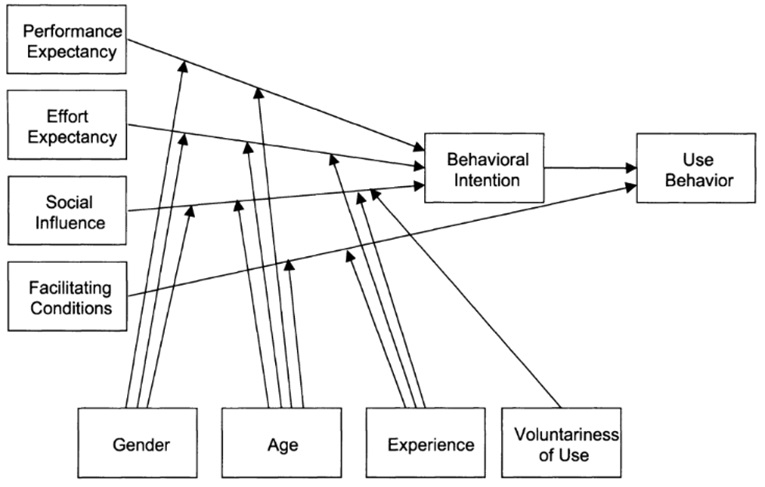
\includegraphics[width=0.7\linewidth]{UTAUT.jpg}
    \captionof{figure}{Original UTAUT Model}
    \label{fig:UTAUT}
        
\end{figure*}
\\By applying UTAUT to the domain of self-custody wallets—a key aspect of financial system digitization that promotes peer-to-peer interactions without intermediaries—the thesis is positioned to dissect the factors propelling technology adoption. As mentioned earlier, this research follows in the footsteps of recent studies that have expanded UTAUT to include additional constructs relevant to blockchain technology adoption, thereby enriching the model's predictive capability in this field (\cite{alazab_blockchain_2021, arias-oliva_fuzzy_2021, ferri_ascertaining_2021, khazaei_integrating_2020, liang_what_2021, queiroz_blockchain_2021, queiroz_blockchain_2019, tran_co-creating_2021, wong_unearthing_2020}).

Before proceeding with a comprehensive literature review, it is beneficial to delve deeper into the definitions and technical aspects of blockchain and its applications. This foundational understanding provides crucial context for analyzing user adoption factors and focusing on self-custody in blockchain-based payments. By elucidating these technical dimensions, we can better appreciate the innovative mechanisms driving blockchain technology as a transformative financial solution.

\subsection{Blockchain Technology and Its Development}

The introduction of Bitcoin in 2009 marked the advent of cryptocurrencies as a viable means of payment \cite{nakamoto_bitcoin_2009}. Following Bitcoin, other blockchains such as Ethereum, XRP, and Binance Coin emerged, each with unique governance models and consensus mechanisms. At its core, blockchain technology is characterized by several major features underpinning its revolutionary potential in the financial sector. Permissionless blockchain ecosystems, such as those exemplified by Bitcoin, are notable for their properties of distributed consensus, immutability, and irreversibility (\cite{moniruzzaman_examining_2020}). These features ensure that once consensus among all participants is met, transactions are recorded on the blockchain and cannot be altered or deleted, thereby providing a secure and transparent ledger of all activities.

The importance of decentralized governance, closely tied to the consensus mechanism, cannot be overstated in blockchain technology. Central to this is whether there is a single point of failure or a centralized authority that can unilaterally make decisions for the entire network. Most prominent blockchain networks adopt the following governance models: on-chain governance, characteristic of Bitcoin (BTC); off-chain governance, as seen in Ethereum (ETH); or a combination of off-chain and on-chain governance mechanisms, as characterized by Binance Coin (BNB) and XRP (\cite{rochard_bitcoin_2020, lee_analysis_2023, noauthor_ethereum_2023, noauthor_governance_2023}). Off-chain governance operates through an informal process of social discussion, whereas on-chain governance relies on the consensus among blockchain validators.

Regarding consensus mechanisms, in permissionless blockchains like Bitcoin and Ethereum, any individual can validate transactions under common conditions, signifying a higher degree of decentralization. This stands in contrast to networks like XRP and Binance Coin, where a central authority selects validators, indicating a potential for greater centralization.

The original blockchain consensus mechanism, known as the Nakamoto consensus protocol, assumes that participants will act in their own best interest. It uses a reward and punishment system to encourage good behavior. Following the rules earns rewards, while breaking them costs money. This makes it more profitable for participants to be honest than to cheat, ensuring the network's integrity without needing to trust each individual (\cite{wang_survey_2019}). This approach not only preserves the integrity of the system but also enhances its resistance to various threats. The transparency and inclusivity of Bitcoin's Proof of Work (PoW) mechanism make its governance highly decentralized, as miners effectively vote on proposed changes by choosing to install or withhold new software features. This decentralized approach is critical to maintaining the security and integrity of the blockchain (\cite{rochard_bitcoin_2020}).

The immutability of blockchain is ensured by its consensus mechanism, where all participants hold an exact copy of the same ledger, making it impossible to alter any single record without majority agreement. This feature guarantees that the data recorded on the blockchain is accurate and trustworthy. 

The distributed ledger, called a blockchain, typically constitutes a chain of blocks of transaction data. Each block contains valid transaction records for a specific period and their attributes, including a key attribute: the timestamp. Blocks are chained together by incorporating a digital fingerprint of the previous block (a hash) into the current block. Any change in the transaction information in a specific block would alter this fingerprint, irreparably breaking the chain of consensus linking that block with all subsequent ones. Consequently, a blockchain functions as both a large-scale, distributed database and an immutable audit trail, where the DNA of each block is incorporated into all following ones, making it impossible to alter history without detection (\cite{catalini_simple_2019}).

Irreversibility in blockchain means that once data is written on the ledger, it cannot be overwritten. This permanence ensures that the historical record remains intact and unchangeable, as any attempt to alter past records would require altering all subsequent blocks, which is practically infeasible due to the need for consensus among all participants (\cite{maurer_when_2013}).

Additionally, blockchain transactions can be conducted peer-to-peer within seconds or minutes, regardless of geographical location, provided there is an internet connection (\cite{wust_you_2018}). This capability significantly enhances the speed and efficiency of financial transactions, bypassing the delays and costs associated with conventional banking systems. 

Bitcoin's blockchain integrates security techniques such as hash chains, Merkle trees, and digital signatures with consensus mechanisms. This combination prevents double spending and inhibits the retrospective modification of transaction data once a block is added to the blockchain. Furthermore, blockchains like Bitcoin are tamper-resistant and resistant to Distributed Denial-of-Service (DDoS) attacks (\cite{zhang_security_2020}). However, utilizing blockchain for secure distributed storage demands additional security and privacy measures.

Permissionless blockchains also mitigate privacy risks because no single entity has preferential access to or visibility over network-generated information. In traditional platforms, intermediaries often access and monetize consumer data, which is increasingly relevant due to its use in AI algorithm training. While blockchain protocols can be designed to offer participants a high degree of privacy (e.g., Zk-Stark, Zcash, Monero), users can also take measures to protect their privacy, such as using mixing services or not reusing addresses. However, shared ledgers like Bitcoin are pseudonymous, allowing third parties to deanonymize transactions over time (\cite{catalini_simple_2019}).

Together, abovementioned features enable self-custody or independent ownership, where users can manage and safeguard their digital assets without relying on third parties.

\subsection{Self-Custody in Blockchain Technology}
\label{subsec:sc}

Self-custody is a fundamental aspect of blockchain technology, allowing users to directly own and manage their digital assets without relying on intermediaries such as banks, exchanges, or other financial institutions (\cite{pimentel_systemizing_2021}). This capability grants users enhanced control, security, privacy, and financial sovereignty over their digital assets. Control over funds in self-custody wallets is ensured by asymmetric or public-key cryptography. In blockchains like Bitcoin, to spend bitcoins, the owner must prove ownership of the private key by digitally signing the transaction. This process guarantees that only the person with the private key can generate a specific signature (\cite{fernandez-carames_towards_2020}).

Self-custody provides users with full ownership of their digital assets, granting them financial sovereignty. Users are not subject to the policies and restrictions of traditional financial institutions. Blockchain's decentralized design protects users from monopoly pricing, as competition among service providers and free entry prevent any single entity from controlling transaction fees. Instead, a market for transaction processing determines the fees users pay to prioritize and avoid delays (\cite{huberman_monopoly_2021}).

However, self-custody also necessitates a thorough understanding of the technology and associated risks, affirming the adage that with greater freedom comes greater responsibility. This responsibility manifests in several key challenges. As it was noted before, users bear sole accountability for managing their private keys, risking permanent loss of assets if keys are lost or forgotten (\cite{eskandari_first_2015}). The absence of traditional customer support means users must rely on community resources and self-education to resolve issues (\cite{conti_survey_2018}). Those lacking technical knowledge may be vulnerable to security risks like hacking and phishing, which also apply to other digital services such as mobile and internet banking (\cite{li_survey_2020}). Moreover, self-custody complicates estate planning and asset inheritance (\cite{katuk_cryptocurrency_2023}).

The characteristics and core values of blockchain and self-custody pave the way for exploring the adoption of self-custodial solutions. By considering factors related to these specificities, we aim to analyze the factors influencing users' adoption of self-custodial solutions using the UTAUT framework.


\subsection{Extended UTAUT Model for Self-Custody Adoption}

A literature review was conducted to establish the empirical foundation for this UTAUT-based study. The search parameters included scientific articles' abstracts, keywords, and titles containing the phrases "technology acceptance" and "blockchain," "technology acceptance" and "crypto," "technology acceptance" and "self-custody," as well as "technology acceptance" and "bitcoin," to determine the relevance of UTAUT constructs for blockchain and self-custody contexts. From 161 articles identified, 10 empirical studies employing the UTAUT framework in the blockchain context were selected for in-depth analysis (see Appendix \ref{app1}). These studies consistently confirmed the significance of the core UTAUT constructs in influencing Behavioral Intention (BI) toward blockchain adoption.

However, scholars have noted that traditional technology acceptance models, including UTAUT, may not fully capture the complexities inherent in adopting highly innovative and decentralized technologies like blockchain (\cite{alomari_factors_2023}; \cite{lampo_how_2022}). Specifically, self-custody introduces unique challenges and responsibilities for users, as outlined in \ref{subsec:sc}, which existing constructs may not fully address. Therefore, extending the UTAUT model with additional constructs could help enhance its explanatory power and offer a more nuanced understanding of self-custody and blockchain adoption (\cite{chang_acceptance_2022}; \cite{ng_factors_2021}).

From the analyzed articles, it became evident that Trust and Security were frequently included alongside original UTAUT constructs in the studies reviewed. Despite identifying five studies in our literature review that emphasize the role of Trust in technology adoption (\cite{aranyossy_konzisztens_2021, baltruschat_user_2023, kabir_application_2021, kumari_impact_2022, chang_acceptance_2022}), and three articles highlighting the significance of Security (\cite{chang_acceptance_2022, radic_you_2022, baltruschat_user_2023}), we have decided not to include these constructs in our research on self-custody adoption in blockchain technology for reasons explained in the following sections.

Trust is a multifaceted concept that spans various dimensions, including interpersonal trust, institutional trust, and trust in technology (\cite{mayer_integrative_1995}; \cite{gambetta_can_1988}; \cite{rheu_systematic_2021}). Exploring Trust comprehensively requires significant depth, given its various roles and types, which fall beyond the scope of our current study. For instance, \textcite{aranyossy_konzisztens_2021} analyzed Perceived Trust across diverse entities like technology and organizations, emphasizing context-specific interpretations of Trust. Similarly, \textcite{baltruschat_user_2023} examined Trust within centralized banking systems, which is less applicable to decentralized blockchain self-custody.

Trust also plays a central role in the adoption of various technologies, such as mobile banking and digital payment platforms (\cite{khalilzadeh_security-related_2017, alalwan_factors_2017, chandra_evaluating_2010, liu_empirical_2017}). However, its inclusion may not add significant explanatory power in the context of self-custody adoption, as blockchain operates on a trust-minimized framework that fundamentally differs from these systems. Blockchain shifts trust from centralized entities to cryptographic proofs and decentralized consensus mechanisms (\cite{nakamoto_bitcoin_2009}; \cite{auinger_blockchain_2018}; \cite{de_filippi_blockchain_2020}). For example, \textcite{chang_acceptance_2022} conflated the concepts of Trust and Transparency, defining the former as the extent to which an individual believes that blockchain-based data and services are accurate, secure, and conducted with full visibility — a perspective that contrasts with the "trustless" nature of blockchain self-custody.

Additionally, trust in technology or code, though relevant, applies universally to digital systems and is not unique to blockchain self-custody. While users need confidence in cryptographic protocols, these are designed to operate without conventional Trust.

Given Trust's broad applicability and complexity, including it may dilute the focus on constructs uniquely relevant to self-custody. Therefore, we have opted not to include it in our model, recognizing it as a complex construct meriting independent study. By focusing on self-custody-specific factors, we provide clearer insights into adoption behaviors in the decentralized blockchain context.

Furthermore, the Security construct is not included in the current study for two primary reasons. First, the literature review did not reveal any studies that link Security directly to BI; instead, they associate it with various other constructs (\cite{baltruschat_user_2023, radic_you_2022, chang_acceptance_2022}). Second, Security is undoubtedly important, but like the Trust construct it is not a differentiating factor for blockchain and self-custody. It might divert attention from concepts that are particularly relevant to self-custody. Implications of Security are critical across all digital technologies (\cite{cimperman_analyzing_2016, khalilzadeh_security-related_2017, widyanto_safety_2022}). The focus is to unravel constructs that specifically highlight and accentuate how blockchain and self-custody differentiate digital money within the realm of blockchain from traditional mobile payment systems, thus offering a more nuanced understanding of blockchain technology's unique adoption factors.

Therefore, the current study focuses on established UTAUT constructs and incorporates additional ones that may play a role in self-custody adoption. Building on the fundamental principles, features, and challenges of self-custody discussed in previous chapters, it is reasonable to assume that decision-making related to self-custody usage stems from these elements. Furthermore, such decision-making likely hinges on users' technical awareness and confidence in their ability to manage digital assets independently. 

First, \textbf{Technology Awareness (TA)} is integrated within the broader construct of Facilitating Conditions (FC), as it considers the users' ability to comprehend the technical intricacies of blockchain systems and effectively manage self-custody wallets (\cite{abubakar_moderating_2013}). Given the complexity of private key management and the absence of third-party support, users must possess a high level of TA to navigate self-custody systems securely. \textcite{kaal_custody_2021} and \textcite{jaroucheh_crypto_2023} highlight the complexity and responsibility of self-custody, noting the necessity of user control over their digital assets, which reduces reliance on third-party custodians. This study proposes incorporating TA into FC, emphasizing its importance in enhancing security, managing digital assets efficiently, and potentially boosting adoption rates.

Next, the study includes \textbf{Personal Innovativeness in the Domain of Internet Technology (PIIT)} to gauge how individual openness to new technologies influences the acceptance of self-custody wallets (\cite{agarwal_conceptual_1998}). Users who are more innovative and comfortable with technology are more likely to embrace the responsibility and control that self-custody demands. Within the realm of blockchain, particularly self-custody in permissionless networks, the technology's complexity necessitates a profound understanding and active engagement from its users. Individuals with elevated levels of PIIT may be more inclined to embrace and utilize innovations like blockchain technology (\cite{boateng_understanding_2023, panjaitan_users_2023}). This construct reflects an individual's openness toward new technological experiences (\cite{mani_consumer_2018}) and is speculated to be instrumental in the diffusion and acceptance of nascent technologies (\cite{khazaei_integrating_2020}). Such innovators and early adopters, characterized by their personal innovativeness, could be instrumental in amplifying blockchain's advantages and propelling its acceptance across a broader audience (\cite{salcedo_effects_2021}).

Lastly, \textbf{Perceived Control (PC)} is introduced to examine how users' belief in their ability to control outcomes impacts their willingness to adopt self-custody solutions (\cite{skinner_guide_1996}). In a system where users are solely responsible for their digital assets, PC plays a critical role in shaping confidence in managing these assets effectively. The concept of holding private keys, as articulated by \textcite{kaal_custody_2021}, is a direct expression of PC, providing users with agency over their digital wallets and assets. \textcite{vadlamani_bridging_2023} suggest that the increasing preference for self-custodial wallets within the DeFi sphere could be due to their promise of heightened privacy, usability, and control, potentially reinforcing the sense of PC among users. Similarly, \textcite{jaroucheh_crypto_2023} posit that self-custody offers users the advantage of transacting without intermediaries, further solidifying their control over digital assets.

The current Thesis proposes that the TA incoporated in FC, PIIT, and PC constructs may significantly impact the adoption of self-custody blockchain wallets. These constructs represent the users' propensity to engage with new technologies, their understanding of the security and management of digital assets, and their sense of autonomy over blockchain transactions. The investigation seeks to validate the theoretical assumption that these constructs are critical influencers, hypotheses that will be examined in depth in the following sections.

\begin{figure*}[tp]
    \centering
    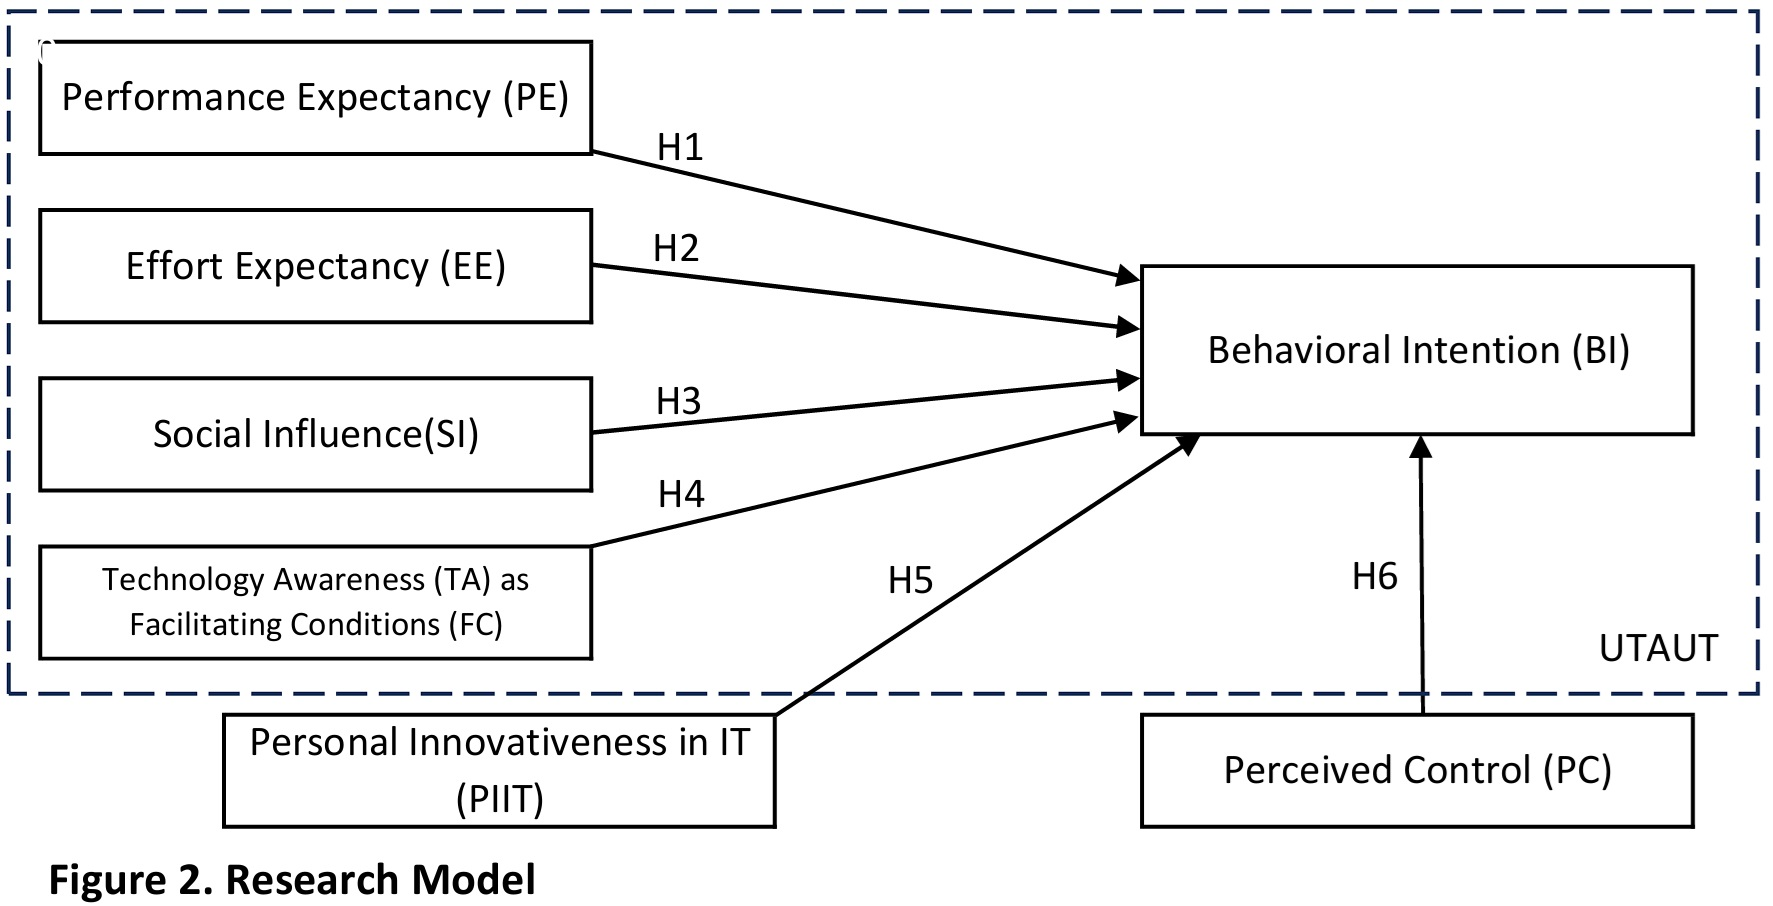
\includegraphics[width=0.9\linewidth]{Research Model.jpg}
    \captionof{figure}{Research Model}
    \label{fig:Model}
       
\end{figure*}

Building upon the UTAUT framework and the additional constructs (TA, PIIT, and PC), this study focuses solely on Behavioral Intention (BI) as the dependent variable, measuring users' likelihood of adopting self-custody wallets. This approach aligns with recent UTAUT-based blockchain studies (\cite{chang_acceptance_2022}, \cite{queiroz_blockchain_2019}) that emphasize BI as a key indicator of technology acceptance, treating actual Use Behavior as a downstream effect rather than a primary focus.

Besides, this research includes traditional UTAUT moderators of gender and age, while omitting experience and voluntariness of use. This selective approach to moderators is supported by \textcite{dwivedi_re-examining_2019}, who noted that most UTAUT studies employ only a subset of moderators based on their contextual relevance. The exclusion of voluntariness of use is justified by the nature of self-custody adoption, which is inherently an individual choice rather than a mandated technology implementation. Given the nascent nature of blockchain technology, where users might have experimented with and discontinued usage of self-custody solutions, traditional experience measures may be less relevant. Therefore, experience as a moderator was substituted with direct measurement of blockchain knowledge, providing a more precise assessment of users' technological understanding.

In summary, the proposed research model comprises BI as the dependent variable, with the core UTAUT constructs (PE, EE, SI, FC) and the additional constructs (PIIT, TA, PC) serving as independent variables. This tailored approach aims to provide a more focused and context-specific understanding of self-custody wallet adoption in the blockchain domain.

\subsubsection{Performance Expectancy (PE)}
PE is a construct that measures an individual's belief in the performance gains from using a system. \textcite{arias-oliva_fuzzy_2021} and \textcite{ferri_ascertaining_2021} have identified PE as a significant factor in the acceptance of cryptocurrencies and blockchain usage in auditing, respectively. \textcite{queiroz_blockchain_2019} also recognized PE's influence on blockchain adoption within supply chain management. Based on these insights, the following hypothesis is proposed:

\textbf{\textit{H1: PE positively influences the BI to adopt self-custody wallets.
}}
\subsubsection{Effort Expectancy (EE)}
EE gauges the perceived ease associated with the use of a system. As evidenced by studies across multiple sectors, it has emerged as a significant factor influencing technology adoption. \textcite{queiroz_blockchain_2021} highlighted its criticality in the context of Brazil's operations and supply chain management, \textcite{ferri_ascertaining_2021} noted its significance in the adoption of blockchain for auditing, and \textcite{arias-oliva_fuzzy_2021} identified it as influential in the intention to use cryptocurrencies. Accordingly, the following hypothesis is proposed:

\textbf{\textit{H2: EE positively influences the BI to adopt self-custody wallets.
}}
\subsubsection{Social Influence (SI)}
SI measures the degree to which an individual perceives that important others believe she or he should use the new system. \textcite{kabir_application_2021} and \textcite{queiroz_blockchain_2019} identified SI as a crucial factor in blockchain-based supply chain management. Additionally, \textcite{ferri_ascertaining_2021} recognized SI as a key predictor of auditors' intention to use blockchain. SI also significantly influences the intention to adopt cryptocurrency payments, especially in South Korea and China, as noted by \textcite{radic_you_2022}. Based on these findings, it is proposed:

\textbf{\textit{H3: SI positively influences the BI to adopt self-custody wallets.
}}

\subsubsection{Facilitating Conditions (FC)}
FC describe the degree to which an individual believes that adequate support is available for using a system. In the blockchain context, the influence of FC has been highlighted in several studies. \textcite{chang_acceptance_2022} identified FC as key to promoting blockchain acceptance among Jeju's residents and visitors. \textcite{queiroz_blockchain_2021} and \textcite{queiroz_blockchain_2019} found FC to be crucial in the adoption of blockchain within supply chain operations. Furthermore, \textcite{radic_you_2022} affirmed that FC significantly influences intentions to use cryptocurrency payments.

We extended the Facilitating Conditions construct to include Technology Awareness (TA). This integration is based on the premise that a deeper understanding of the technology not only facilitates its usage but also enhances the overall conditions that support its adoption. TA specifically contributes to FC by providing users with the knowledge and insights necessary to effectively manage and utilize technology, thereby reducing barriers to adoption (\cite{abubakar_moderating_2013}). This approach acknowledges that users who are more aware of and knowledgeable about the specifics of blockchain and self-custody are better equipped to leverage these technologies to their full potential. By incorporating TA into the FC construct, we aim to capture the role of informed awareness in promoting an environment conducive to adopting new technologies.

Based on these insights, the following hypothesis is proposed:

\textbf{\textit{H4: FC positively influences the Behavioral Intention (BI) to adopt self-custody wallets.}}


\subsubsection{Personal Innovativeness in the Domain of Internet Technology (PIIT)}

UTAUT has been instrumental in evaluating technology adoption within organizational contexts. However, its application can be limited regarding individual consumer behavior in non-organizational settings. This is particularly relevant in scenarios where technology adoption is a matter of personal choice rather than an institutional directive (\cite{venkatesh_consumer_2012}). \textcite{dwivedi_re-examining_2019} further critiques the UTAUT model for its lack of consideration for individual traits like personal innovativeness, which can significantly sway an individual's decision to accept and use new technologies.
\\Self-custody wallet adoption is largely an individual's decision, necessitating a more tailored approach than the UTAUT model traditionally offers. To better capture this individual adoption behavior, PIIT is introduced into the model. PIIT measures how open or inclined a person is towards adopting new IT innovations, independent of the specific organizational context in which the individual operates (\cite{agarwal_conceptual_1998}). PIIT is vital for understanding the adoption of self-custody solutions, where individuals independently manage their digital assets. The relevance of such a construct is supported by findings from \textcite{ng_factors_2021}, who demonstrated that innovativeness is a pertinent factor in understanding how individuals, such as buyers and sellers in the real estate sector, accept blockchain technology. Therefore, the following hypothesis is posited:

\textbf{\textit{H5. PIIT positively affects the BI to adopt self-custody wallets.
}}

\subsubsection{Perceived Control (PC)}
To further refine the adaptation of the UTAUT for studying self-custody wallet adoption, Perceived Control (PC) was introduced as an additional construct. \textcite{skinner_guide_1996} highlighted control as the individuals' belief in their ability to achieve desired outcomes, a critical driver in technology adoption. Specifically, individuals who perceive a high degree of control over technology are more likely to hold positive attitudes toward its use (\cite{ajzen_perceived_2002}). \textcite{rocha_role_2018} demonstrated this in a study in Jordan, which showed that the intention to adopt smart meters was influenced by providing users with control over their electricity consumption data. This factor is particularly relevant in the context of self-service technologies (SSTs), where the perception of control can decisively influence continued use or abandonment after a service failure (\cite{le_perceived_2022}).
\\ \textcite{lin_dcap_2020} emphasize the importance of PC over outcomes in the marketing and consumer behavior fields, particularly regarding new product adoption. \textcite{liu_empirical_2017} found that PC influenced the continued intention to use Apple Pay, while \textcite{cabinakova_understanding_2019} noted its stronger impact on users of blockchain-based decentralized identity management systems compared to centralized ones.
\\By integrating PC into the model, this study aims to assess how the sense of control over self-custody affects the adoption of blockchain wallets, providing deeper insights into the drivers of technology acceptance. Hence, the hypothesis is:

\textbf{\textit{H6. PC positively affects the BI to adopt self-custody wallets.
}}

\section{Methodology}
Building on the Unified Theory of Acceptance and Use of Technology, the research seeks to understand the factors driving the adoption of self-custody crypto wallets. The study serves an exploratory function by investigating a relatively new phenomenon while also employing an analytical approach to examine the relationships between well-defined variables. The choice of UTAUT as a foundation is deliberate, given its comprehensive nature and proven efficacy in technology adoption studies. By integrating constructs like PIIT, PC, and TA the aim is to provide a more holistic view of the adoption dynamics, especially in the context of self-custody. To achieve this, the ways of selecting participants, gathering information, and analyzing the data are carefully designed to match the study's framework. Furthermore, research instruments from prior studies are adopted, modified, and tailored to fit the research model, ensuring their relevance and effectiveness in the specific research context.

\subsection{Research Design}
The research design serves as a roadmap for the study, guiding the selection of the blockchain network, the development of the research instrument, and the choice of analytical approach. Given blockchain technology's nascent and dynamic nature, selecting a network that epitomizes decentralization, acceptance, and practicality is imperative. As detailed later, the preliminary analysis zeroes in on the Bitcoin network, which aligns with the research model's focus on decentralization and widespread adoption.

\subsubsection{Selection of Blockchain Network for Research Analysis}

Given the varying attributes of blockchains, the current research focuses on the network that offers the utmost decentralization, widespread acceptance, significant capitalization, and reasonable fees. A preliminary analysis was conducted on five leading networks by market capitalization: Bitcoin (BTC), Ethereum (ETH), Binance Coin (BNB), Tether (USDT), and XRP (XRP), based on market data from \href{https://www.coinmarketcap.com}{CoinMarketCap} as of August 23, 2023. However, Tether was excluded due to its reliance on other networks. The evaluation criteria encompassed the degree of decentralization, market capitalization, acceptance, and transaction fees.
\\The governance models and consensus mechanisms were identified as significant determinants of a blockchain's decentralization level (\cite{noauthor_ethereum_2023}; \cite{noauthor_governance_2023}; \cite{lee_analysis_2023}; \cite{rochard_bitcoin_2020}). Among the evaluated networks, Bitcoin and Ethereum emerged as more decentralized, being permissionless blockchains, compared to BNB and XRP. Transaction fees were also a notable factor (\cite{noauthor_bitcoin_2023}; \cite{noauthor_bitcoin_2023-1}), with BNB and XRP offering lower fees (\cite{noauthor_binance_2023}; \cite{noauthor_xrp_2023}), but at the potential cost of centralization (\cite{christodoulou_consensus_2020}; \cite{maksymyuk_blockchain-empowered_2022}; \cite{thomas_how_2017}).
\\A detailed comparative analysis (refer to Appendix \ref{app2}) revealed Bitcoin as the most suitable network for the research, given its unparalleled decentralization, market dominance, and reasonable transaction fees (\cite{davis_cryptocurrency_2023}; \cite{flynn_how_2022}; \cite{mallqui_predicting_2019}; \cite{vejacka_basic_2014}). Despite Ethereum's decentralization and versatility, its higher transaction fees made it less preferable. The centralization concerns of BNB and XRP rendered them less suitable for the current decentralization-focused research.
\\Considering Bitcoin's global acceptance and its embodiment of a decentralized blockchain network, the study will primarily focus on the Bitcoin network as the archetypal blockchain-based payment system. 

\subsubsection{Sampling design and data collection}

The research employs a quantitative approach, utilizing an online survey methodology. The target demographic encompasses individuals from diverse backgrounds, including public and private sector employees, students, and current or former users of self-custody blockchain wallets. The survey will be distributed using several channels, including LinkedIn, Telegram, Reddit posts, Twente University Startup Community Slack Channel, X (former Twitter) tweets, Nostr notes, and among Technical University Berlin student WhatsApp groups. To further enhance the reach and diversity of respondents, specialized survey exchange platforms such as www.surveyswap.com and www.surveycircle.com will also be utilized. These platforms facilitate reciprocal survey participation among researchers and participants, potentially broadening the demographic scope of the study.

This multi-platform distribution ensures a diverse respondent pool and mitigates potential biases. The strategy aligns with Convenience Sampling, a non-probability sampling method that selects participants based on accessibility and convenience (\cite{lavrakas_nonprobability_2008}). While this method facilitates efficient data collection, it may introduce biases related to the self-selection of participants and the non-randomness of the sample, which are acknowledged and will be considered in the analysis.

Furthermore, as participants in the initial sample might share the survey within their networks, a Snowball Sampling effect is expected, where new participants are continuously referred. This method is often used in studies with specific target groups (\cite{goodman_snowball_1961}). 

By employing these sampling methods, the aim is to gather insights from a wide array of participants engaged with blockchain technology, while being mindful of the limitations and potential biases these methods introduce. The analysis will
consider these factors, aiming to provide a balanced and comprehensive understanding of the adoption of self-custody blockchain wallets.


\begin{table*}[pb]
\centering
\small
\caption{Survey Instrument (latent variables)}
\label{tab:survey_instrument}
\begin{tabular}{@{}p{1.7cm}p{0.7cm}p{10cm}p{3.8cm}@{}} 
\toprule
\textbf{Construct}                        & \textbf{Code} & \textbf{Indicators} & \textbf{Adapted from} \\ \midrule
Performance Expectancy                    & PE1           & How useful do you find using a self-custody Bitcoin wallet for managing your Bitcoin transactions? & \textcite{venkatesh_user_2003, venkatesh_consumer_2012} \\  (PE)
                                          & PE2           & Do you believe using a self-custody Bitcoin wallet can help you accomplish tasks more effectively when storing and transacting your Bitcoin? & \textcite{queiroz_blockchain_2019} \\
                                          & PE3           & In your opinion, can using a self-custody Bitcoin wallet improve your productivity in storing and transacting your Bitcoin? &  \\
                                          & PE4           & How strongly do you agree that using a self-custody Bitcoin wallet will enhance your financial performance? &  \\
\\Effort Expectancy                       & EE1           & How strongly do you agree that interacting with a self-custody Bitcoin wallet is clear and understandable? & \textcite{venkatesh_user_2003, venkatesh_consumer_2012} \\
(EE)                                      & EE2           & How strongly do you agree that becoming skillful at using a self-custody Bitcoin wallet is easy for you? & \textcite{wong_unearthing_2020} \\
                                          & EE3           & How strongly do you agree that you find a self-custody Bitcoin wallet easy to use? &  \\
                                          & EE4           & How strongly do you agree that learning how to use a self-custody Bitcoin wallet is easy? &  \\
\\Social Influence                        & SI1           & People who influence my behavior believe I should use a self-custody Bitcoin wallet. & \textcite{albayati_accepting_2020} \textcite{venkatesh_user_2003} \\
 (SI)                                     & SI2           & People who are important to me think I should use a self-custody Bitcoin wallet. &  \textcite{queiroz_blockchain_2019} \\
                                          & SI3           & Influential figures in the cryptocurrency community endorse using self-custody Bitcoin wallets. &  \\
                                          & SI4           & The widespread adoption of self-custody Bitcoin wallets in my community would influence my decision to use one. &  \\
\\Facilitating                            & FC1           & I read news and other resources about self-custody Bitcoin wallets. & \textcite{dinev_centrality_2007}  \\
Conditions (FC)(+TA)                      & FC2           & I discuss the security and technical aspects of self-custody Bitcoin wallets with peers or within my network. &  \textcite{venkatesh_user_2003} Queiroz and Fosso Wamba \\
                                          & FC3           & Self-custody Bitcoin wallets are not compatible with other systems I use. (This is a reverse-coded item) & (2019) \\
                                          & FC4           & I can obtain assistance from others when I encounter difficulties with a self-custody Bitcoin wallet. &  \\
\\Personal Innovative-                    & PIIT1         & When new technologies become available, I seek ways to experiment with them. & \textcite{agarwal_conceptual_1998} \\
ness in IT (PIIT)                         & PIIT2         & I am often the first among my peers to use new technologies like self-custody Bitcoin wallets. & \textcite{leong_predicting_2013} \\
                                          & PIIT3         & I am generally reluctant to use new technologies such as self-custody Bitcoin wallets. (This is a reverse-coded item) &  \\
                                          & PIIT4           & I actively engage in exploring new technologies like self-custody Bitcoin wallets. &  \\
\\Perceived Control                       & PC1           & I feel I have control over managing and securing my Bitcoin when using a self-custody wallet without interference from third parties. & \textcite{taylor_understanding_1995}, \textcite{cabinakova_understanding_2019} \\
(PC)                                      & PC2           & Using a self-custody Bitcoin wallet, my Bitcoin is within my control. &  \\
\\Behavioral                              & BI1           & I intend to use a self-custody Bitcoin wallet in the future. & Venkatesh et al. (2003,  \\
Intention                                 & BI2           & I will always try to use a self-custody Bitcoin wallet in my daily life. & 2012) \\
(BI)                                      & BI3           & I plan to use a self-custody Bitcoin wallet frequently. \\ \bottomrule
\end{tabular}
\end{table*}

\subsubsection{Instrument Development}

The survey instrument, detailed in Table \ref{tab:survey_instrument}, is developed based on previous literature to measure seven distinct constructs through a total of 25 items, ensuring that the content domain of each construct is thoroughly covered (\cite{agarwal_conceptual_1998, venkatesh_consumer_2012, venkatesh_user_2003, queiroz_blockchain_2019, wong_unearthing_2020, albayati_accepting_2020, dinev_centrality_2007, leong_predicting_2013, taylor_understanding_1995, cabinakova_understanding_2019}). Besides the latent constructs from UTAUT, the model uses additional variables such as PIIT and PC. 

PE measures users' perceived benefits of self-custody Bitcoin wallets through four items, drawing from \textcite{queiroz_blockchain_2019} and \textcite{venkatesh_user_2003, venkatesh_consumer_2012}. EE evaluates the ease with which users can learn and use these wallets based on four items from \textcite{venkatesh_user_2003, venkatesh_consumer_2012} and \textcite{wong_unearthing_2020}. SI captures the effect of influential individuals and community consensus on users' adoption decisions, adapted from \textcite{albayati_accepting_2020}, \textcite{queiroz_blockchain_2019}, and \textcite{venkatesh_user_2003}, via four items. 

FC evaluates the accessibility of resources, knowledge, and support necessary for utilizing the wallets, as defined by \textcite{queiroz_blockchain_2019} and \textcite{venkatesh_user_2003, venkatesh_consumer_2012}. In our study, we combined FC with Technology Awareness (TA) (\cite{dinev_centrality_2007}) to capture a more comprehensive view of the facilitating factors specific to blockchain and self-custody wallet adoption. This adaptation, consisting of four items, aims to assess not only the availability of resources and support but also the user's awareness and understanding of the technology, which we hypothesized to be crucial in the context of self-custody wallets.

PIIT possibly offers insights into individual tendencies to adopt new technologies. \textcite{agarwal_conceptual_1998} and \textcite{ng_factors_2021} both accentuated the significance of PIIT in identifying early adopters and understanding technology acceptance dynamics. 

In the current context, PC feasibly plays a pivotal role in technology adoption. As delineated by \textcite{taylor_understanding_1995}. PC is bifurcated into two primary dimensions: self-efficacy, representing an individual's confidence in executing a behavior, and conditions representing resources availability to engage in behavior. In the study, these dimensions are encapsulated by indicators PC1 and PC2. This approach ensures a comprehensive representation of PC while also maintaining survey brevity and respondent engagement.

As already mentioned, the focus on BI sidelining Use Behavior is in sync with blockchain-centric studies like \textcite{radic_you_2022}, \textcite{chang_acceptance_2022}, and \textcite{queiroz_blockchain_2019}, all of which prioritize intention over actual use. \textcite{venkatesh_user_2003, venkatesh_consumer_2012} further consolidate the importance of BI, emphasizing its role as a determinant in the UTAUT framework. In this research, BI, represented by BI1 and BI2, captures the intent of users toward the adoption of self-custody Bitcoin wallets.

The survey employs a 7-point Likert scale for twenty five questions, ranging from 'strongly disagree' to 'strongly agree.' Additionally, four demographic and two knowledge questions are incorporated to categorize the criteria (Table \ref{tab:demographics}).


\begin{table}[H]
\centering
\small
\caption{Demographic and Knowledge indicators (control variables)}
\label{tab:demographics}
\begin{tabular}{p{2.5cm}p{5cm}}
\hline
\textbf{Item}                                         & \textbf{Value} \\ \hline
Gender                                                & Female \\
                                                      & Male \\
                                                      & Non-Binary/Other \\
                                                      & I prefer not to say \\
\\                                                    & 18-25 \\
                                                      & 26-33 \\
Age                                                   & 34-41 \\
                                                      & 42-49 \\
                                                      & 50+ \\
\\                                                    & No formal education \\
                                                      & Primary \\
                                                      & Secondary \\
Highest Educa-                                        & Diploma / Polytechnic \\
tion Level                                            & Bachelor's degree \\
                                                      & Postgraduate degree (Master's/Ph. D.) \\
\\                                                    & Banking \\
                                                      & Financial Institutional \\
                                                      & IT Related \\
                                                      & Manufacturing \\
Industry                                              & Retail \\
                                                      & Telecommunication \\
                                                      & Tourism \\
                                                      & Education \\
                                                      & Other \\
\\Who has access                                        & Only the Wallet Provider \\
to the funds                                          & Only the Wallet Owner \\
stored in a self-                                     & The Wallet Provider and Owner \\
custody wallet?                                       & Bank 
\\                                                    & I don't know \\
 \hline
\end{tabular}
\end{table}

Demographic Questions could be essential as they provide context to the responses and allow for segmentation during data analysis. The questions on Gender, Age, Highest Education Level, and Industry are comprehensive and will help understand the respondents' background.

Knowledge Question may provide crucial insight into respondents' understanding of self-custody wallets, particularly regarding control and access to funds. This approach may offer a more precise evaluation of users' technological comprehension than mere usage duration, especially relevant for emerging technologies like blockchain where actual understanding may vary regardless of experience.

The chosen sample and method align with the research goal and question. The sample, comprising individuals from diverse backgrounds, ensures a broad spectrum of perspectives, capturing the multifaceted nature of blockchain adoption. This diversity is crucial, given the universal appeal and applicability of blockchain. The method, rooted in the UTAUT model, is tailored to delve deep into the intricacies of technology adoption, making it apt for the study. Including constructs like PIIT and PC, along with extending FC to incorporate TA, further aligns the method with the research goal, ensuring a comprehensive exploration of the factors driving blockchain adoption.

A small-scale pilot survey will be conducted using the initial version of the questionnaire. This pilot phase is crucial in gathering feedback to ensure the reliability and relevance of the questions (\cite{brace_questionnaire_2004}). Based on the insights gained from this pilot survey, necessary adjustments will be made to improve clarity and effectiveness. The questions will be carefully crafted to avoid bias and guarantee respondent anonymity. Following these refinements, the final questionnaire will be distributed to a broader audience for data collection. After gathering the data, a demographic analysis will be performed to assess the representativeness of the sample, and any potential limitations in the findings will be transparently discussed.

\subsection{Data analysis}

The analysis employed multiple regression, specifically an ordinal logistic regression to explore the relationships between the independent variables and the dependent variable (Behavioral Intention to adopt self-custody wallets), alongside demographic and background variables. This method, as outlined by \textcite{cohen_applied_2003}, allows for the assessment of the relative impact of each predictor on end-users adoption intentions.
The ordinal logistic regression model, also known as the proportional odds model, is particularly advantageous for our study for several reasons. Firstly, unlike linear regression, it is robust to non-normal distribution, which makes it suitable for our non-normally distributed data. Secondly, it effectively handles ordinal data, respecting the ordinal nature of our Behavioral Intention (BI) construct, which is composed of 3 Likert-scale indicators. Lastly, this model doesn't assume equal distances between ordinal categories, which is appropriate for Likert-scale data. (\cite{hair_multivariate_2019, cohen_applied_2003})

The conceptual model underlying our analysis can be represented by the following equation:

\begin{align}
BI = & \, \beta_0 + \beta_1(\text{PE}) + \beta_2(\text{EE}) + \beta_3(\text{SI}) + \beta_4(\text{FC}) \nonumber \\
     & + \beta_5(\text{PIIT}) + \beta_7(\text{PC}) + \beta_8(\text{Gender}) + \beta_9(\text{Age}) \nonumber \\
     & + \beta_{10}(\text{Education}) + \beta_{11}(\text{Industry}) \nonumber \\
     &  + \beta_{12}(\text{Knowledge})+ \epsilon
\end{align}

Where:
\begin{itemize}
    \item \(BI\) = Behavioral Intention to adopt self-custody wallets.
    \item \(PE\) = Performance Expectancy.
    \item \(EE\) = Effort Expectancy.
    \item \(SI\) = Social Influence.
    \item \(FC\) = Facilitating Conditions.
    \item \(PIIT\) = Personal Innovativeness in the Domain of Internet Technology.
    \item \(PC\) = Perceived Control.
    \item Gender, Age, Education, Industry, and Knowledge represent the demographic and background variables, encoded appropriately.
    \item \(\beta_0\) = Intercept.
    \item \(\beta_1\) to \(\beta_{12}\) = Coefficients for each predictor, indicating the size and direction of the relationship between the predictor and the dependent variable.
    \item \(\epsilon\) = Error term, capturing the variation in BI not explained by the model.
\end{itemize}

In this equation, BI represents the Behavioral Intention to adopt self-custody wallets (composite score from 3 indicators), $\beta_0$ is the intercept, $\beta_1$ to $\beta_12$ are the coefficients for each predictor, and $\epsilon$ is the error term. PE, EE, SI, FC, PIIT, and PC are the main predictor variables, while Gender, Age, Education, Industry, and Knowledge represent the demographic and background variables, encoded appropriately.


\subsection{Addressing bias and validity issues}

Mitigating potential biases and confirming the validity of the findings are crucial steps in ensuring the integrity of the research. A series of preliminary checks and analyses will be conducted to ensure the quality and appropriateness of our data and measures. First, we will perform a reliability analysis, calculating Cronbach's alpha, and ensuring consistent measurement across items (\cite{eisinga_reliability_2013}). This will be followed by an Exploratory Factor Analysis (EFA), as recommended by \textcite{costello_best_2005}, to clarify the data structure and provide insights into the constructs' interrelations. We will then examine the correlation matrix to understand the relationships between variables and check for potential multicollinearity issues. To further address multicollinearity concerns, we will calculate Variance Inflation Factors (VIFs) for all predictor variables (\cite{mukaka_guide_2012}). These preliminary steps will ensure the robustness of our subsequent analysis and help in interpreting the results accurately.


\section{Results}

This section presents a comprehensive analysis of our results on the adoption of self-custody crypto wallets. We begin with an overview of the sample characteristics, followed by a detailed examination of the measurement validation process. Subsequently, we present the findings from our regression model, which investigates the factors influencing the behavioral intention to adopt self-custody wallets.

\subsection{Descriptive Statistics}

Our study encompassed a diverse sample of 131 respondents, providing a rich dataset for analysis (Table \ref{tab:descriptive_stats}). The sample demographics reveal a balanced gender distribution, with a slight male majority (50\%, n=66). Notably, the educational background of the participants was skewed towards higher education, with 80\% holding at least a Bachelor's degree, including a substantial proportion (40\%, n=53) with postgraduate qualifications. These findings may be particularly relevant for understanding self-custody wallet adoption among educated professionals and early adopters (\cite{van_rijnsoever_effect_2009}) but should be cautiously generalized to broader populations with diverse educational backgrounds.


\begin{table}[ht!]
\centering
\caption{Descriptive Statistics}
\label{tab:descriptive_stats}
\resizebox{\columnwidth}{!}{%
\begin{tabular}{llcc}
\toprule
\textbf{Item} & \textbf{Values} & \textbf{Freq.} & \textbf{Perc.} \\
\midrule
\textbf{Source of } & Facebook & 8 & 6\% \\
\textbf{Questionnaire} & Flyers & 1 & 1\% \\
 & LinkedIn & 7 & 5\% \\
 & Nostr & 2 & 2\% \\
 & Reddit & 17 & 13\% \\
 & Survey Platform & 38 & 29\% \\
 & Telegram & 3 & 2\% \\
 & Viber & 1 & 1\% \\
 & WhatsApp & 53 & 40\% \\
 & X & 1 & 1\% \\
\midrule
\textbf{Gender} & Female & 62 & 47\% \\
 & Male & 66 & 50\% \\
 & Non-binary & 3 & 2\% \\
\midrule
\textbf{Age} & 18-25 & 44 & 34\% \\
 & 26-33 & 55 & 42\% \\
 & 34-41 & 14 & 11\% \\
 & 42-49 & 12 & 9\% \\
 & 50+ & 6 & 5\% \\
\midrule
\textbf{Education} 
 & Secondary & 13 & 10\% \\
 & Diploma / Polytechnic & 13 & 10\% \\
 & Bachelor's degree & 52 & 40\% \\
 & Postgraduate (Master/Ph.D.) & 53 & 40\% \\
\midrule
\textbf{Field of Work} & Banking & 8 & 6\% \\
 & Education & 8 & 6\% \\
 & Financial Institution & 8 & 6\% \\
 & IT Related & 33 & 25\% \\
 & Manufacturing & 7 & 5\% \\
 & Other & 53 & 40\% \\
 & Retail & 9 & 7\% \\
 & Telecommunication & 2 & 2\% \\
 & Tourism & 3 & 2\% \\
\midrule
\textbf{Knowledge Question} & Bank & 4 & 3\% \\
Who has access & I don't know & 44 & 34\% \\
to the funds stored & Only the wallet owner & 69 & 53\% \\
in self-custody wallet? & Only the wallet provider & 4 & 3\% \\
 & Wallet provider and owner & 10 & 8\% \\
\bottomrule
\end{tabular}
}
\end{table}

In terms of professional background, Information Technology (IT) roles were the most common specified field, accounting for 27\% (n=34) of the sample. However, the largest group (38\%, n=48) identified their field as 'Other', indicating a wide variety of industries not specifically listed.

Regarding knowledge about self-custody wallets, 53\% (n=69) correctly identified that only the wallet owner has access to the funds. However, a significant portion (34\%, n=44) were unsure about access to funds in self-custody wallets.

WhatsApp proved to be the most effective platform for survey distribution, accounting for 40\% (n=53) of responses, followed by dedicated Survey Platforms (29\%, n=38) and Reddit (13\%, n=17).

This diverse sample provides a broad perspective on the adoption of self-custody crypto wallets, with a particular emphasis on young, educated professionals across various fields, notably in technology-related industries.


\subsection{Measurement Validation}

The reliability analysis conducted through R statistical computing environment showed that most constructs demonstrated strong internal consistency, with one notable exception. Constructs such as EE, PE, BI, and PC exhibit high reliability, each with a Cronbach's alpha above 0.8. Specifically, EE has a Cronbach's alpha of 0.884, with item-total correlations ranging from 0.732 to 0.765, indicating strong internal consistency. PE similarly shows a Cronbach's alpha of 0.84, with item-total correlations between 0.616 and 0.804, confirming the robustness of the scale. BI also demonstrates strong reliability, with a Cronbach's alpha of 0.878 and item-total correlations ranging from 0.683 to 0.820. PC exhibits a Cronbach's alpha of 0.802, with very high item-total correlations, further underscoring its reliability.

In contrast, constructs such as SI and PIIT demonstrate moderate reliability, with Cronbach's alpha values between 0.7 and 0.8. SI has a Cronbach's alpha of 0.797, though it is worth noting that item SI4 had a lower item-total correlation. PIIT shows a Cronbach's alpha of 0.735, with generally good item-total correlations. However, PIIT3 exhibited a weaker correlation, which may be attributed to the fact that this item was reverse-coded. 

\begin{table}[ht!]
\centering
\caption{Comparison of Cronbach's Alpha and Item-Total Correlations Before and After Excluding FC3}
\label{tab:alpha_r_cor_comparison}
\resizebox{\columnwidth}{!}{%
\begin{tabular}{lcccccc}
\toprule
\textbf{Scale} & \textbf{Item} & \textbf{Original} & \textbf{Revised} & \textbf{Original} & \textbf{Revised} & \textbf{Change} \\
 &  & \textbf{$\alpha$} & \textbf{$\alpha$} & \textbf{$r_{\text{cor}}$} & \textbf{ $r_{\text{cor}}$} & \textbf{in $r_{\text{cor}}$} \\
\midrule
\textbf{PE} & PE1 & 0.840 & 0.840 & 0.688 & 0.688 & 0.000 \\
                                   & PE2 &      &      & 0.889 & 0.889 & 0.000 \\
                                   & PE3 &      &      & 0.830 & 0.830 & 0.000 \\
                                   & PE4 &      &      & 0.581 & 0.581 & 0.000 \\
\midrule
\textbf{EE} & EE1 & 0.884 & 0.884 & 0.777 & 0.777 & 0.000 \\
                               & EE2 &      &      & 0.817 & 0.817 & 0.000 \\
                               & EE3 &      &      & 0.814 & 0.814 & 0.000 \\
                               & EE4 &      &      & 0.779 & 0.779 & 0.000 \\
\midrule
\textbf{SI} & SI1 & 0.797 & 0.797 & 0.915 & 0.915 & 0.000 \\
                              & SI2 &      &      & 0.892 & 0.892 & 0.000 \\
                              & SI3 &      &      & 0.594 & 0.594 & 0.000 \\
                              & SI4 &      &      & 0.416 & 0.416 & 0.000 \\
\midrule
\textbf{FC(+TA)} & FC1 & 0.534 & 0.730 & 0.756 & 0.772 & +0.016 \\
                                     & FC2 &      &      & 0.768 & 0.764 & -0.004 \\
                                     & FC3 &      & (Excluded) & -0.097 & (Excluded) & -- \\
                                     & FC4 &      &      & 0.454 & 0.441 & -0.013 \\
\midrule
\textbf{PIIT} & PIIT1 & 0.735 & 0.735 & 0.665 & 0.665 & 0.000 \\
                                           & PIIT2 &      &      & 0.786 & 0.786 & 0.000 \\
                                           & PIIT3 &      &      & 0.287 & 0.287 & 0.000 \\
                                           & PIIT4 &      &      & 0.805 & 0.805 & 0.000 \\
\midrule
\textbf{PC} & PC1 & 0.802 & 0.802 & 0.747 & 0.747 & 0.000 \\
                               & PC2 &      &      & 0.747 & 0.747 & 0.000 \\
\midrule
\textbf{BI} & BI1 & 0.878 & 0.878 & 0.717 & 0.717 & 0.000 \\
                                  & BI2 &      &      & 0.867 & 0.867 & 0.000 \\
                                  & BI3 &      &      & 0.885 & 0.885 & 0.000 \\
\bottomrule
\end{tabular}%
}
\smallskip
\begin{flushleft}
\footnotesize \textbf{Note}: Only the \textit{Facilitating Conditions} scale was modified by excluding item \textbf{FC3}. All other scales remain unchanged.
\end{flushleft}
\end{table}


This issue is even more pronounced in the FC scale, which presents significant reliability concerns with a Cronbach's alpha of only 0.534. Notably, item FC3, also reverse-coded, showed a negative item-total correlation and a negative correlation with the first principal component. This suggests that FC3 may not align well with the overall construct.

Given these findings, we decided to conduct a comparative reliability analysis of the FC scale with and without FC3. The results of this analysis are presented in Table \ref{tab:alpha_r_cor_comparison}, allowing for a clear assessment of the impact of FC3 on the scale's overall reliability. 

Exploratory Factor Analysis (EFA) was conducted to assess the dimensionality of the measurement scales. While parallel analysis suggested a three-factor solution, we also examined a seven-factor solution to align with our theoretical constructs. In both solutions, item FC3 from the Facilitating Conditions scale demonstrated problematic characteristics.

In the three-factor solution, FC3 did not load significantly on any factor (all loadings $< 0.3$), indicating that it does not align well with the overall factor structure. In the seven-factor solution, FC3 showed only a weak negative loading (-0.324) on one factor.

These EFA results corroborate the earlier reliability analysis, where FC3 was found to have a negative item-total correlation within the Facilitating Conditions scale (Cronbach's alpha = 0.534). The negative loading and correlation suggest that FC3 may be conceptually opposite to what the Facilitating Conditions scale aims to measure. This aligns with findings from \textcite{queiroz_blockchain_2019}, who also reported lower outer loadings for this item (0.685). 

Given these consistent indications across multiple analyses, we decided to remove item FC3 from further analysis. This decision is expected to improve the overall reliability and validity of the Facilitating Conditions construct, as well as enhance the clarity of the factor structure in our measurement model.

\begin{table*}[ht]
\centering
\caption{Means, Standard Deviations, and Correlations of the Variables}
\label{tab:correlation_matrix}
\begin{tabular}{lccccccccc}
\toprule
\textbf{Variable} & \textbf{Mean} & \textbf{S.D.} & \textbf{PE} & \textbf{EE} & \textbf{SI} & \textbf{FC} & \textbf{PIIT} & \textbf{PC} & \textbf{BI} \\
\midrule
\textbf{PE}   & 4.66 & 1.29 & 1.00 &       &       &       &       &       \\
\textbf{EE}   & 4.36 & 1.31 & 0.59 & 1.00  &       &       &       &       \\
\textbf{SI}   & 4.35 & 1.37 & 0.67 & 0.57  & 1.00  &       &       &       \\
\textbf{FC(+TA)}   & 3.64 & 1.51 & 0.47 & 0.49  & 0.61  & 1.00  &       &       \\
\textbf{PIIT} & 4.04 & 1.30 & 0.44 & 0.51  & 0.45  & 0.54  & 1.00  &       \\
\textbf{PC}   & 4.83 & 1.54 & 0.55 & 0.64  & 0.53  & 0.57  & 0.57  & 1.00  \\
\textbf{BI}   & 3.99 & 1.62 & 0.61 & 0.59  & 0.67* & 0.69** & 0.60** & 0.55  & 1.00 \\
\bottomrule
\end{tabular}
\smallskip
\begin{flushleft}
\footnotesize \centering ** Correlation is significant at the 0.01 level (2-tailed). \\
* Correlation is significant at the 0.05 level (2-tailed).
\end{flushleft}
\end{table*}

The correlation matrix (Table \ref{tab:correlation_matrix}) reveals key insights into the relationships between constructs influencing the Behavioral Intention (BI) to adopt self-custody crypto wallets. All correlations are positive, with the strongest being between FC and BI (0.69), followed by SI and BI (0.67). PIIT also shows a strong correlation with BI (0.60). PE and EE have moderately strong correlations with BI (0.61 and 0.59 respectively). Among independent variables, PE and SI show the highest correlation (0.67). No correlations exceed 0.7, reducing concerns about severe multicollinearity. 

Additionally, Variance Inflation Factors (VIFs) for all predictors in our ordinal regression model were calculated. VIF values greater than 5 are often considered concerning, while values above 10 indicate severe multicollinearity issues  (\cite{cohen_applied_2003}).

Most of our predictors show VIF values well below the threshold of concern, ranging from 1.48 (PIIT) to 2.52 (PC) for our main constructs. This suggests that multicollinearity is not a major issue for these variables.
However, two categorical variables show elevated VIF values: Age (VIF = 5.52)and Industry (VIF = 5.78). The GVIF values, which adjust for the degrees of freedom of each variable, are all below 1.6, further suggesting that multicollinearity is not a severe issue in our model.


\subsection{Regression Model}

Using R for statistical analysis, an ordinal logistic regression was conducted to examine factors influencing Behavioral Intention (BI) to adopt self-custody wallets  (\cite{christensen_ordinal_2023, venables_modern_2010}). The model demonstrated a strong overall fit ($\chi^2$ = 162.225, df = 27, p $<$ 0.001; Table \ref{tab:modelfit}), meaning that the probability of getting such a good fit by chance alone is very small. The deviance value was 322.92. The model's explanatory power is evidenced by multiple R² measures: McFadden's R² (0.334) indicates a reasonable fit; typically, values between 0.2 and 0.4 suggest that the model is performing well in explaining the data. Additionally, Nagelkerke R² (0.728) and Cox \& Snell R² (0.710) suggest strong predictive capability. The model achieved a classification accuracy of 48.1\%, substantially exceeding the random chance for a seven-point ordinal outcome.

The analysis proceeded in two stages. First, a baseline model incorporating only demographic and background variables was estimated. Second, theoretical predictors were added both individually and collectively to assess their incremental contribution.

\begin{table}[htbp]
\centering
\caption{Model Fit Statistics for Full Model}
\label{tab:modelfit}
\begin{tabular}{lr}
\hline
Statistic & Value \\
\hline
Log-Likelihood & -161.459 \\
AIC & 388.918 \\
BIC & 483.799 \\
McFadden R² & 0.334 \\
Nagelkerke R² & 0.728 \\
Cox \& Snell R² & 0.710 \\
Classification Accuracy & 0.481 \\
Likelihood Ratio $\chi^2$ (df = 27) & 162.225*** \\
\hline
\multicolumn{2}{l}{\small Note: ***p $<$ 0.001} \\
\end{tabular}
\end{table}

The model estimated six threshold parameters (zeta) for the ordinal outcome levels: 1|2 (4.39), 2|3 (6.67), 3|4 (8.37), 4|5 (10.60), 5|6 (12.54), and 6|7 (14.45), all showing statistical significance (p $<$ 0.001), meaning that the model successfully distinguishes between different levels of intention, further validating its fit.

The Baseline Model, incorporating only demographic and background variables, revealed several significant predictors of behavioral intention (BI) to adopt self-custody crypto wallets (Table \ref{tab:summary_ordinal_logit}). Age emerged as a significant factor, with the 42-49 age group showing a negative association (B = -1.53, p $<$ 0.05) and the 50+ age group demonstrating a positive relationship (B = 2.01, p $<$ 0.05) with BI. 

Education level also played a role, with postgraduate degree holders exhibiting a significant negative association (B = -1.20, p $<$ 0.01) compared to other education levels. Industry affiliation showed mixed effects, with participants from the education (B = -2.94, p $<$ 0.01) and manufacturing (B = -2.90, p $<$ 0.01) sectors demonstrating significantly lower BI compared to other industries.

To assess the incremental explanatory power of each theoretical construct, we added individual independent variables (IVs) to the baseline model. All six IVs demonstrated significant positive associations with BI when added individually to the baseline model. Facilitating Conditions (FC) exhibited the strongest effect (B = 1.18, p $<$ 0.001), followed by Personal Innovativeness in IT (PIIT) (B = 1.13, p $<$ 0.001), Social Influence (SI) (B = 1.05, p $<$ 0.001), Performance Expectancy (PE) (B = 1.00, p $<$ 0.001), Effort Expectancy (EE) (B = 0.96, p $<$ 0.001), and Perceived Control (PC) (B = 0.77, p $<$ 0.001).

Notably, the inclusion of individual IVs generally maintained the significance of demographic factors identified in the baseline model, particularly age and industry effects, but remarkable changes occurred with some IVs. Both PE and EE, while highly significant in their individual models (p $<$ 0.001), lost their significance in the full model (PE: B = 0.38, p $>$ 0.05; EE: B = 0.32, p $>$ 0.05). This suggests that their effects might be mediated by other variables, particularly FC and PIIT, which maintained their significance in the full model.

Perhaps the most striking transformation occurred with Perceived Control (PC). While PC showed a significant positive effect when tested individually (B = 0.77, p $<$ 0.001), it not only lost significance but also reversed direction in the full model (B = -0.20, p $>$ 0.05). This unexpected reversal suggests that PC's influence on adoption intention may be conditional on other factors, particularly FC, TA and PIIT. When technical support (FC), technical (TA) and individual capability (PIIT) are accounted for, PC may become redundant or even counterproductive in predicting adoption intentions.

The full model revealed varying effects of theoretical predictors on adoption intention (Table \ref{tab:hypotheses}). Facilitating Conditions showed the strongest effect (OR = 2.085, 95\% CI [1.429, 3.078], p $<$ 0.001), indicating that a one-unit increase in FC more than doubles the odds of higher adoption intention. Personal Innovativeness in IT demonstrated the second strongest effect (OR = 1.989, 95\% CI [1.347, 2.965], p $<$ 0.001), followed by Social Influence (OR = 1.527, 95\% CI [1.025, 2.291], p $<$ 0.05).

Contrary to our expectations (H1 and H2), Performance Expectancy (OR = 1.466, 95\% CI [0.945, 2.278], p = 0.087) and Effort Expectancy (OR = 1.379, 95\% CI [0.906, 2.113], p = 0.135) did not significantly affect adoption intention. This suggests that when accounting for other factors, the perceived usefulness and ease of use may not be primary drivers of adoption intention.

H3 was supported, as Social Influence (SI) maintained a significant positive effect on BI (B = 0.42, p $<$ 0.05), albeit with a reduced coefficient compared to the individual IV model, increasing adoption odds by about 53\% per unit increase (OR = 1.527). This indicates that social norms and peer influence play a role in adoption decisions, even when controlling for other factors.

The analysis of Hypothesis 4 (H4) supported the significant role of Facilitating Conditions (FC), enhanced by the integration of Technology Awareness (TA) elements. The odds ratio indicates that improving FC by one unit more than doubles the likelihood of higher adoption intention. This strong effect suggests that users' intention to adopt self-custody wallets is heavily influenced by both technical support infrastructure and their understanding of blockchain technology's fundamental principles. 

\clearpage
\begin{landscape}
\begin{table}[htbp]
\centering
\caption{Coefficients for Different Models}
\label{tab:summary_ordinal_logit}
\resizebox{\linewidth}{!}{%
\begin{tabular}{@{}lrrrrrrrrrrrrrrrr@{}}
\toprule
& \multicolumn{2}{c}{Baseline Model} & \multicolumn{2}{c}{\shortstack{Baseline Model\\+ PE}} & \multicolumn{2}{c}{\shortstack{Baseline Model\\+ EE}} & \multicolumn{2}{c}{\shortstack{Baseline Model\\+ SI}} & \multicolumn{2}{c}{\shortstack{Baseline Model\\+ FC(+TA)}} & \multicolumn{2}{c}{\shortstack{Baseline Model\\+ PIIT}} & \multicolumn{2}{c}{\shortstack{Baseline Model\\+ PC}} & \multicolumn{2}{c}{Full Model} \\ 
\cmidrule(lr){2-3} \cmidrule(lr){4-5} \cmidrule(lr){6-7} \cmidrule(lr){8-9} \cmidrule(lr){10-11} \cmidrule(lr){12-13} \cmidrule(lr){14-15} \cmidrule(lr){16-17}
Predictor & B & s.e. & B & s.e. & B & s.e. & B & s.e. & B & s.e. & B & s.e. & B & s.e. & B & s.e. \\
\midrule
GenderMale & 0.486 & 0.374 & 0.616 & 0.369 & 0.616 & 0.380 & 0.334 & 0.375 & 0.281 & 0.394 & -0.223 & 0.404 & 0.247 & 0.382 & 0.038 & 0.435 \\
GenderNon-Binary & 0.932 & 1.433 & 1.779 & 1.429 & 0.953 & 1.343 & 1.868 & 1.637 & -0.038 & 1.453 & 0.421 & 1.182 & 1.441 & 1.379 & 0.523 & 1.355 \\
Age26-33 & -0.459 & 0.459 & -0.159 & 0.470 & -0.348 & 0.475 & -0.613 & 0.477 & 0.042 & 0.506 & 0.144 & 0.472 & -0.331 & 0.457 & 0.211 & 0.512 \\
Age34-41 & 0.071 & 0.665 & 0.275 & 0.682 & -0.320 & 0.681 & -0.083 & 0.650 & -0.140 & 0.697 & 0.277 & 0.694 & -0.503 & 0.693 & 0.105 & 0.733 \\
Age42-49 & -1.535* & 0.734 & -1.460 & 0.748 & -1.806* & 0.764 & -1.968* & 0.790 & -1.388 & 0.812 & -1.574* & 0.767 & -1.669* & 0.784 & -1.767* & 0.828 \\
Age50+ & 2.006* & 0.856 & 1.520 & 0.866 & 2.561** & 0.923 & 1.046 & 0.885 & 1.103 & 0.903 & 1.942* & 0.909 & 2.021* & 0.858 & 1.120 & 0.962 \\
EducationDiploma / Polytechnic & 0.826 & 0.741 & 1.334 & 0.773 & 1.491 & 0.798 & 1.240 & 0.785 & 1.223 & 0.785 & 1.199 & 0.749 & 1.194 & 0.776 & 1.798* & 0.808 \\
EducationPostgraduate degree & -1.205** & 0.411 & -0.899* & 0.416 & -0.749 & 0.421 & -0.822* & 0.419 & -0.952* & 0.413 & -0.984* & 0.424 & -1.061* & 0.415 & -0.462 & 0.436 \\
EducationSecondary & -1.101 & 0.640 & -0.537 & 0.654 & -0.461 & 0.657 & -0.383 & 0.641 & 0.188 & 0.672 & -0.666 & 0.640 & -0.457 & 0.635 & 0.411 & 0.699 \\
IndustryEducation & -2.937** & 0.990 & -2.862** & 0.992 & -2.765** & 1.001 & -2.582* & 1.052 & -2.585* & 1.012 & -3.758*** & 1.017 & -2.141* & 1.036 & -3.514** & 1.083 \\
IndustryFinancial Institution & 0.549 & 0.951 & 0.304 & 0.918 & -0.005 & 0.971 & -0.047 & 0.970 & -0.113 & 0.946 & 0.259 & 0.935 & 1.094 & 0.963 & -1.077 & 1.000 \\
IndustryIT Related & -0.017 & 0.759 & 0.004 & 0.740 & -0.359 & 0.768 & -0.189 & 0.758 & 0.012 & 0.768 & 0.294 & 0.749 & 0.798 & 0.803 & -0.333 & 0.790 \\
IndustryManufacturing & -2.896** & 1.015 & -1.314 & 1.030 & -2.850** & 1.031 & -2.154* & 1.047 & -1.389 & 1.046 & -2.830** & 1.063 & -1.322 & 1.077 & -1.571 & 1.161 \\
IndustryOther & -0.893 & 0.747 & -0.907 & 0.737 & -1.016 & 0.744 & -0.899 & 0.739 & -0.367 & 0.732 & -1.085 & 0.735 & -0.379 & 0.782 & -0.980 & 0.744 \\
IndustryRetail & 0.224 & 0.948 & -0.503 & 0.968 & -0.233 & 0.970 & -0.237 & 0.954 & 1.164 & 0.989 & 0.259 & 0.941 & 0.811 & 0.982 & 0.120 & 0.994 \\
IndustryTelecommunication & 2.712 & 1.734 & 1.818 & 1.613 & 1.385 & 1.665 & 2.185 & 1.627 & 1.194 & 1.657 & 1.891 & 1.626 & 3.073 & 1.623 & 0.444 & 1.806 \\
IndustryTourism & -1.941 & 1.293 & -2.188 & 1.384 & -1.910 & 1.416 & -1.252 & 1.306 & -1.151 & 1.229 & -1.478 & 1.329 & -0.851 & 1.359 & -1.284 & 1.264 \\
KnowledgeI don't know & -0.519 & 0.943 & -0.436 & 0.948 & -0.235 & 0.985 & -0.391 & 1.035 & 0.146 & 0.933 & -0.290 & 0.940 & -1.105 & 0.965 & 0.364 & 1.014 \\
KnowledgeOnly the wallet owner & 1.095 & 0.959 & 0.529 & 0.958 & 0.573 & 1.000 & 0.616 & 1.045 & 1.536 & 0.945 & 0.994 & 0.954 & -0.526 & 1.024 & 1.195 & 1.084 \\
KnowledgeOnly the wallet provider & 1.309 & 1.289 & 1.119 & 1.222 & 0.908 & 1.297 & 1.270 & 1.343 & 1.030 & 1.373 & 1.151 & 1.220 & -0.082 & 1.355 & 1.229 & 1.329 \\
KnowledgeThe wallet provider and owner & -0.556 & 1.163 & -0.374 & 1.161 & -0.336 & 1.231 & -0.835 & 1.240 & 0.205 & 1.153 & -0.336 & 1.171 & -1.684 & 1.207 & 0.227 & 1.289 \\
PE & & & 1.005*** & 0.170 & & & & & & & & & & & 0.383 & 0.223 \\
EE & & & & & 0.964*** & 0.171 & & & & & & & & & 0.321 & 0.215 \\
SI & & & & & & & 1.054*** & 0.165 & & & & & & & 0.424* & 0.205 \\
FC(+TA) & & & & & & & & & 1.181*** & 0.165 & & & & & 0.735*** & 0.195 \\
PIIT & & & & & & & & & & & 1.131*** & 0.179 & & & 0.688*** & 0.200 \\
PC & & & & & & & & & & & & & 0.767*** & 0.160 & -0.200 & 0.206 \\
\midrule
\multicolumn{17}{c}{Intercepts} \\
\midrule
1|2 & -4.089** & 1.287 & 0.139 & 1.497 & -0.434 & 1.469 & -0.555 & 1.482 & 0.441 & 1.379 & -0.296 & 1.391 & -1.331 & 1.434 & 4.391** & 1.654 \\
2|3 & -2.632* & 1.244 & 1.890 & 1.482 & 1.254 & 1.447 & 1.333 & 1.463 & 2.236 & 1.358 & 1.657 & 1.377 & 0.387 & 1.418 & 6.667*** & 1.669 \\
3|4 & -1.566 & 1.232 & 3.159* & 1.493 & 2.480 & 1.454 & 2.698 & 1.479 & 3.679** & 1.389 & 2.986* & 1.397 & 1.576 & 1.421 & 8.366*** & 1.727 \\
4|5 & -0.036 & 1.217 & 4.951** & 1.512 & 4.222** & 1.463 & 4.525** & 1.489 & 5.638*** & 1.433 & 4.788*** & 1.421 & 3.217* & 1.423 & 10.602*** & 1.787 \\
5|6 & 1.219 & 1.219 & 6.457*** & 1.549 & 5.734*** & 1.500 & 6.038*** & 1.522 & 7.291*** & 1.485 & 6.257*** & 1.452 & 4.594** & 1.443 & 12.536*** & 1.876 \\
6|7 & 2.365 & 1.247 & 7.843*** & 1.610 & 7.153*** & 1.564 & 7.442*** & 1.580 & 8.964*** & 1.594 & 7.681*** & 1.521 & 5.906*** & 1.496 & 14.454*** & 2.011 \\
\bottomrule
\end{tabular}%
}
\smallskip
\begin{flushleft}
\footnotesize \centering Note: * p $<$ 0.05, ** p $<$ 0.01, *** p $<$ 0.001
\end{flushleft}
\end{table}
\end{landscape}


Specifically, the modified FC construct captured users' access to resources and knowledge necessary for wallet management, along with their awareness of blockchain's decentralized nature and self-custody implications. However, it's important to note that these results should be interpreted with caution due to measurement adaptations and reliability concerns, which are addressed in the study's limitations.

\begin{table*}[ht]
\centering
\caption{Summary of Hypotheses Testing Results}
\label{tab:hypotheses}
\begin{tabular}{llcll}
\hline
Hypothesis & Path & Odds Ratio & 95\% CI & Result \\
\hline
H1 & PE → BI & 1.466 & [0.945, 2.278] & Not Supported \\
H2 & EE → BI & 1.379 & [0.906, 2.113] & Not Supported \\
H3 & SI → BI & 1.527* & [1.025, 2.291] & Supported \\
H4 & FC(+TA) → BI & 2.085*** & [1.429, 3.078] & Supported \\
H5 & PIIT → BI & 1.989*** & [1.347, 2.965] & Supported \\
H6 & PC → BI & 0.818 & [0.545, 1.228] & Not Supported \\
\hline
\multicolumn{5}{l}{\small Note: *p $<$ 0.05, ***p $<$ 0.001} \\
\end{tabular}
\end{table*}

H5 was also supported, with Personal Innovativeness in IT (PIIT) showing a significant positive effect on BI (B = 0.69, p $<$ 0.001) with the second-highest odds ratio (OR = 1.989). This suggests that individual propensity to embrace new technologies remains a key factor in predicting adoption intentions, even in the presence of other variables.

Contrary to H6, Perceived Control showed a negative, non-significant effect (OR = 0.818, 95\% CI [0.545, 1.228], p = 0.332). This unexpected reversal from its positive effect in the individual model suggests that PC's influence may become redundant or even counterproductive when technical support (FC), technical (TA) and individual capabilities (PIIT) are accounted for.

The full model exhibited improved discriminatory power across all levels of BI, as evidenced by the high significance (p $<$ 0.01 or p $<$ 0.001) of all intercepts.



\section{Discussion}

This study tries to advance our understanding of self-custody cryptocurrency wallet adoption by extending the UTAUT model and uncovering novel insights into the factors influencing users' adoption intentions. While self-custody offers significant advantages through complete asset control and independence from traditional banking constraints, it also presents unique challenges including key management responsibilities, security concerns, and regulatory uncertainties. Despite these complexities, blockchain adoption has been studied across various domains - from supply chain management (\cite{queiroz_blockchain_2019}) to tourism (\cite{radic_you_2022}), healthcare (\cite{baltruschat_user_2023}), and finance (\cite{kumari_impact_2022}) - yet research specifically examining self-custody adoption remains limited. The extension of UTAUT through additional constructs - Technology Awareness (TA) operationalized in Facilitating Conditions (FC), Personal Innovativeness in IT (PIIT), and Perceived Control (PC) - provides a framework for analyzing blockchain technology adoption, particularly in addressing the balance between user autonomy and implementation challenges.

The empirical findings from 131 respondents look to challenge traditional technology adoption paradigms in two significant ways. First, the classical drivers of technology adoption - Performance Expectancy (PE) and Effort Expectancy (EE) - demonstrated non-significance, which can suggest that adoption decisions for complex, highly innovative technologies like blockchain may depend more on users’ access to supportive resources and their awareness of the system's decentralized principles, rather than on perceived ease of use or performance enhancements. Second, an unexpected reverse effect was exhibited concerning Perceived Control (PC): while showing significant positive influence when tested individually, PC became non-significant and slightly negative in the full model. This reversal suggests an interaction effect where PC's influence diminishes when technical support infrastructure and individual capabilities are accounted for.

The analysis reveals that self-custody adoption is primarily driven by a distinct triad of factors: Facilitating Conditions enhanced by Technology Awareness (FC+TA), Personal Innovativeness in IT (PIIT), and Social Influence (SI). This pattern aligns with the fundamental value proposition and unique challenges of self-custody solutions. The significance of FC+TA indicates the primacy of understanding and support infrastructure over perceived usefulness or ease of use. The prominence of PIIT suggests that individuals with higher technological innovativeness demonstrate greater adoption propensity, while SI's significance points to the role of social networks in adoption decisions.

The findings demonstrate that successful adoption of self-custody solutions depends more on building robust support infrastructure and fostering social networks than on emphasizing utility or ease of use. This understanding carries implications for blockchain technology development, implementation strategies, and regulatory frameworks, particularly in addressing the technical and social dimensions of self-custody adoption. These results may provide an empirical foundation for future research examining the evolving landscape of blockchain-based financial solutions.

\subsection{Theoretical Implications}

Our expanded UTAUT model aimed to offer a more nuanced understanding of technology adoption in the blockchain domain. The study shed light on the unique dynamics of self-custody solutions, where traditional constructs of usefulness and ease of use give way to more foundational elements of technological understanding and social support. This shift suggests a more nuanced theoretical framework may be needed when examining technologies that fundamentally alter user-system relationships, particularly those requiring users to assume greater responsibility and autonomy.

The integration of Technology Awareness (TA) within Facilitating Conditions (FC) represents a theoretical advancement in understanding how users approach technologies that challenge established paradigms. While traditional UTAUT constructs focus on operational aspects, the significance of FC+TA suggests that the adoption of transformative technologies requires a deeper cognitive engagement - users must not only understand how to use the technology but also grasp its underlying principles and implications. This finding extends beyond \textcite{kabir_application_2021}'s work in supply chain financing, suggesting that technological awareness becomes particularly crucial when the technology challenges fundamental assumptions about trust, control, and responsibility.

The significant role of PIIT in predicting adoption intentions highlights the importance of individual characteristics in technology acceptance, particularly for innovative technologies. While \textcite{ng_factors_2021} proposed incorporating innovativeness into UTAUT for blockchain adoption studies, it has not been widely implemented in the field. Our results, however, suggest that individual propensity to adopt new technologies is indeed a crucial factor in the context of self-custody, supporting \textcite{ng_factors_2021}'s proposition and demonstrating the value of including PIIT in blockchain adoption models. Regarding our study case adoption requires users to embrace not just new tools, but new paradigms of thinking about ownership, control, and responsibility.

The significant impact of Social Influence (SI) on Behavioral Intention (BI) in our study aligns with previous research in the blockchain domain, such as studies by \textcite{ferri_ascertaining_2021} and \textcite{kumari_impact_2022}. Unlike traditional technologies where SI primarily drives awareness and acceptance, in self-custody solutions, social networks may serve as crucial support systems for managing the increased responsibility and complexity.

Interestingly, the non-significant results for Performance Expectancy (PE) and Effort Expectancy (EE) challenge some traditional assumptions about technology adoption. This diverges from findings in studies like \textcite{baltruschat_user_2023} and \textcite{chang_acceptance_2022}, who found PE to be a significant predictor of blockchain adoption. The findings suggest that when technologies fundamentally alter user autonomy and responsibility, traditional utility-based adoption models may be insufficient. This divergence points to a theoretical gap in understanding how users evaluate technologies that offer not just functional benefits, but transformative changes in their relationship with financial systems.

These findings collectively suggest a need to evolve technology adoption theory beyond its traditional focus on utility and ease of use, particularly for technologies that fundamentally reshape user agency and responsibility. The theoretical framework must expand to account for the interplay between technological understanding, individual readiness for paradigm shifts, and social support systems. This evolution in theoretical understanding may be crucial as technologies increasingly offer not just new capabilities, but new models of user empowerment and responsibility.

\subsection{Practical Implications}

Building upon our theoretical contributions to the UTAUT model in the blockchain context, our findings offer valuable insights for the effective adoption of self-custody wallets across different stakeholders: organizations, individuals, financial service providers' customers, and notably, the education sector. The strong influence of Facilitating Conditions (FC) aided by Technology Awareness (TA), along with the significant roles of Personal Innovativeness in IT (PIIT) and Social Influence (SI), inform a comprehensive approach to implementation.


Our findings provide actionable insights for implementing self-custody solutions, emphasizing the critical role of support systems in driving adoption. The significant influence of Facilitating Conditions (FC) enhanced by Technology Awareness (TA), combined with Personal Innovativeness in IT (PIIT) and Social Influence (SI), demonstrates that successful adoption requires a comprehensive understanding of user behavior and support needs, beyond mere technological infrastructure.

The strong relationship between FC(+TA) and adoption intentions necessitates prioritizing user education beyond basic functionality. For instance, crypto exchanges should integrate mandatory or incentivized educational modules addressing key management, scam prevention, and market manipulation awareness into their onboarding process. Following \textcite{di_nicola_resilient_2020}'s findings on multi-signature systems, these modules should emphasize practical security measures, including backup procedures and emergency protocols, with advanced feature access contingent on demonstrating security competence.

Our model reveals the crucial role of early adopters through significant PIIT effects while highlighting the responsibility to protect these initial users. Following \textcite{buterin_why_2021}'s recommendations on social recovery mechanisms, exchanges and wallet providers should implement graduated access systems, allowing users to practice with test networks before managing significant assets. This protection ensures early adopters maintain positive experiences and effectively guides the early majority through their adoption journey.

The strong effect of SI on adoption intentions underscores the importance of community-driven support networks. Blockchain stakeholders, including mining pools and node operators, should actively participate in user education by providing network security documentation, incentivizing proper security practices, and maintaining dedicated support channels.

The unexpected negative correlation between the education sector and adoption intentions points to a critical gap in blockchain literacy within traditional educational settings. Rather than relying on centralized organizational initiatives, this finding suggests a need for community-driven educational approaches leveraging the open-source nature of blockchain technology. For instance, educators could engage directly with open-source documentation, participate in public development discussions, and contribute to educational resources on platforms like GitHub. This bottom-up approach aligns with blockchain's fundamental principles of decentralization and permissionless innovation. Academic institutions could integrate these community-maintained resources into their curricula, while educators themselves could participate in decentralized autonomous organizations (DAOs) focused on education, contributing their pedagogical expertise to improve blockchain literacy. Such grassroots involvement could transform educators from adoption barriers into active participants in the blockchain ecosystem, organically catalyzing adoption through their understanding and experience with the technology's open-source foundations.

For individual adoption, our findings emphasize the need for progressive learning paths that align with blockchain's open-source nature. Rather than relying on centralized organizations, the adoption of self-custody can be facilitated through existing community channels and network effects. Our finding that Perceived Control (PC) becomes less significant with proper support infrastructure suggests that decentralized knowledge sharing and peer support networks can effectively guide new users. For instance, blockchain foundations already provide comprehensive documentation and guides, but their reach could be amplified through technologically innovative individuals by providing them access to various social channels (SI), where they can contextualize technical information for different audiences and demonstrate practical applications.

Payment infrastructure providers and crypto exchanges currently bridge traditional finance and blockchain technology, but our findings about the significant role of Technology Awareness (TA) within Facilitating Conditions (FC) suggest that mere intermediation may hinder true adoption. Our data shows that understanding blockchain's underlying principles drives adoption more strongly than perceived ease of use or performance benefits (non-significant EE and PE).

The recent approval of Bitcoin and Ethereum ETFs, while expanding institutional access, risks reinforcing traditional custodial models that prioritize convenience over technological understanding. Based on our findings - where technical awareness and direct control prove crucial for adoption - institutional investors should develop robust self-custody protocols through multi-signature schemes and dedicated key management systems, rather than defaulting to third-party custody solutions.

By implementing these strategies, which directly align with our theoretical extensions to the UTAUT model, all stakeholders can more effectively navigate the adoption of self-custody wallets. This multi-faceted approach, emphasizing education, gradual implementation, community support, and leveraging early adopters, addresses all key factors identified in our research. Special attention to the education sector can help overcome the identified adoption barriers and potentially turn this sector into a driving force for blockchain literacy and adoption in the broader society.

\subsection{Policy Implications}

Our findings offer crucial insights for policymakers regarding blockchain and self-custody adoption, particularly in the context of financial democratization and market demonopolization. The significant role of Technology Awareness (TA) in our model suggests that policymakers must first develop a thorough understanding of how self-custody empowers individuals by removing traditional financial intermediaries and returning asset control to users.

Examples from progressive jurisdictions demonstrate how informed policy approaches can foster adoption while protecting consumers. Switzerland's Crypto initiative provides a supportive regulatory environment for blockchain innovation, particularly encouraging self-custody solutions through clear legal frameworks and regulatory certainty. Similarly, El Salvador's adoption of Bitcoin as legal tender, despite implementation challenges, illustrates how government policy can accelerate financial inclusion through blockchain technology.

Our findings about the significance of Personal Innovativeness in IT (PIIT) and Social Influence (SI) suggest that policymakers should support grassroots innovation and community-driven adoption. Rather than imposing traditional financial regulations that may stifle blockchain's democratizing potential, policies should create spaces for experimentation and peer-to-peer learning. This could involve:
\begin{itemize}
   \item Establishing regulatory sandboxes that allow testing of new self-custody solutions while ensuring consumer protection
   \item Supporting community-led educational initiatives that enhance public understanding of blockchain's empowering features
   \item Developing frameworks that recognize and protect individuals' right to self-custody of their digital assets
   \item Creating guidelines that prevent traditional financial institutions from unnecessarily restricting self-custody options
\end{itemize}

The strong influence of Facilitating Conditions (FC) Items in our model suggests that policy frameworks should focus on enabling infrastructure rather than controlling it. This aligns with successful approaches seen in jurisdictions that prioritize innovation while maintaining market integrity. Such policies can help prevent the re-emergence of financial monopolies in the digital asset space while ensuring adequate consumer protection through education and transparency requirements rather than restrictive regulations.

Furthermore, our finding that Performance Expectancy (PE) and Effort Expectancy (EE) are non-significant suggests that policies should focus less on operational efficiency and more on preserving blockchain's fundamental value proposition of financial autonomy. This insight should guide policymakers in developing frameworks that protect users' right to maintain direct control over their assets while ensuring adequate support systems exist for safe self-custody practices.


\subsection{Limitations}

While this study offers valuable insights into self-custody crypto wallet adoption, several limitations warrant consideration. Our research design, which utilized a select set of UTAUT constructs and omitted the Use Behavior component, may have overlooked potentially influential factors. Although this approach aligns with recent blockchain studies (\cite{chang_acceptance_2022,queiroz_blockchain_2019}) by focusing on Behavioral Intention, it does not capture actual usage patterns, potentially limiting our understanding of the full adoption process.

Methodologically, our use of ordinal logistic regression with a composite Behavioral Intention score, while suitable for our study's objectives, may not fully capture the nuanced relationships between predictors and individual BI components. This limitation is compounded by our sample size of 131 participants, which, though acceptable, sits at the lower threshold for a study with six hypotheses. A larger sample could have afforded greater statistical power and potentially uncovered additional significant relationships.

Our research design's focus on select UTAUT constructs, while omitting the Use Behavior component, reflects a common approach in blockchain studies (\cite{chang_acceptance_2022,queiroz_blockchain_2019}). However, this focus on Behavioral Intention without capturing actual usage patterns limits our understanding of the adoption process, particularly in a rapidly evolving technology landscape where intention may not directly translate to sustained use.

The adaptation of the Facilitating Conditions (FC) construct to incorporate technology awareness elements presented unique challenges. This modification, coupled with reliability issues that necessitated the removal of item FC3, may have compromised the construct's comprehensiveness and comparability with studies using the original UTAUT model. 

A significant limitation stems from the inherent characteristics of blockchain technology research. The possible focus on individuals already familiar with self-custody concepts, while providing depth, may restrict the generalizability of our findings to the broader population. Additionally, the decentralized nature of blockchain systems makes it challenging to capture the full spectrum of adoption factors, particularly those related to community-driven development and permissionless innovation.

These limitations underscore the need for future research to employ refined measures, particularly for facilitating conditions, in the context of emerging financial technologies. Subsequent studies would benefit from:
\begin{itemize}
    \item Larger, more diverse samples that better represent the potential user base
    \item Longitudinal designs that capture actual usage patterns over time
    \item More sophisticated analytical approaches, such as Structural Equation Modeling
    \item Improved measurement instruments that better reflect blockchain's decentralized nature
    \item Investigation of adoption patterns across different market conditions and regulatory environments
\end{itemize}

Such efforts would not only confirm and extend our findings but also contribute to a more comprehensive understanding of self-custody wallet adoption in the evolving landscape of blockchain technology.

\subsection{Future Research}

This study's findings open several avenues for future research in self-custody wallet adoption and broader blockchain technology acceptance.

The most intriguing finding requiring further investigation is the shifting role of Perceived Control (PC). While traditionally viewed as crucial in technology adoption, our study found PC becoming non-significant and slightly negative when accounting for other factors. Future research should examine how this relationship evolves as users gain experience with self-custody, and how different implementations of self-custody features affect users' perception of control. This could lead to a fundamental reassessment of how control is conceptualized in blockchain adoption studies.

Similarly unexpected were the non-significant results for Performance Expectancy (PE) and Effort Expectancy (EE), contradicting previous findings in blockchain adoption studies. This suggests a need for comparative research across different blockchain applications to understand when and why traditional adoption factors become less relevant. Longitudinal studies could be particularly valuable in tracking how these relationships evolve as the technology matures and users become more sophisticated.

The significance of Facilitating Conditions (FC) enhanced by Technology Awareness (TA) suggests future research should examine specific aspects of technological support and their impact on adoption. This could include investigating how different forms of blockchain education influence awareness and studying the interaction between technical support and user autonomy in self-custody contexts.

The strong influence of Personal Innovativeness in IT (PIIT) and Social Influence (SI) indicates the need to explore how early adopters and community dynamics influence the broader adoption of self-custody solutions. Understanding these social and individual factors could be crucial for developing effective adoption strategies.

The unexpected negative correlation between the education sector and adoption intention merits deeper investigation, particularly regarding barriers to blockchain literacy in academic institutions and the development of effective educational approaches for self-custody concepts.

Future studies should also consider more sophisticated methodological approaches, including mixed-method designs and cross-cultural studies to examine how adoption factors vary across different contexts. This knowledge will be crucial as blockchain continues to evolve, potentially reshaping traditional financial systems and user relationships with digital assets.




\onecolumn
\clearpage
\addcontentsline{toc}{section}{References}
\printbibliography[title={References}]

\clearpage
\onecolumn
\appendix
\begin{landscape}
\setlength{\tabcolsep}{3pt}
\section{Appendix A: UTAUT Articles Literature Review}
\label{app1}

\vspace{-0.5 cm} 


\begin{longtable}{|p{1.7cm}|p{1.5cm}|p{17.7cm}|p{2.0cm}|}
\caption*{Table \thetable: Summary of Research Articles} \label{tab:research_articles} \\
\hline
\textbf{Author(s)} & \textbf{Prospect} & \textbf{Summary} & Relationship \\
\hline
\endfirsthead

\multicolumn{4}{c}%
{{\bfseries \tablename\ \thetable{} -- continued from previous page}} \\
\hline
\textbf{Author(s)} & \textbf{Prospect} & \textbf{Summary} & Relationship \\
\hline
\endhead

\hline
\multicolumn{4}{r}{{Continued on next page}} \\
\endfoot

\hline
\endlastfoot
\small
\textcite{aranyossy_konzisztens_2021} & Individual Prospect & The article investigates the factors influencing attitudes toward the use of a hypothetical social media cryptocurrency, utilizing the UTAUT framework. Data analysis was conducted through Partial Least Squares Structural Equation Modeling (PLS-SEM), particularly applying the consistent PLS method tailored to their research objectives. Key findings indicate a significant positive relationship between performance expectation (PE) and intention to use (IU), highlighting PE as the most influential factor, ease of use (EoU) and IU, and perceived trust (PT) and IU. & PE → IU \newline EE → IU \newline PT → IU  \\
\hline
\textcite{baltruschat_user_2023} & Individual Prospect & The study examines the user acceptability of blockchain technology for exchanging electronic health records (EHRs). The research analyzed data from 214 participants via a survey and employed partial least squares path modeling for analysis. Key findings indicate that performance expectancy (PE), social influence (SI) positively influence the acceptance of blockchain for EHR sharing, while perceived security (PS) positively influences perceived trust (PT), which in turn positively influences behavioral intention (BI). Practical implications emphasize the need for user understanding of the system's purpose and functions, incentives for sharing health data, and the impact of health personnel on patients' blockchain solution usage. & PE → BI \newline SI → BI \newline PT → BI \newline PS → PT  \\
\hline
\textcite{bozkurt_is_2022} & Individual Prospect & The article investigates the motivations and factors influencing individuals' investments in cryptocurrencies from a behavioral finance perspective. It utilized Structural Equation Modeling (SEM) to analyze data from 216 participants, focusing on the relationships between observed and latent variables within a newly developed model. The main findings highlight that performance expectation (PE) is the most significant factor affecting investment behavior, influencing both the behavioral intention to use blockchain technology and actual investment actions. This suggests that individuals are likely to invest in cryptocurrencies if they perceive it will enhance their performance.  & PE → BI \\
\hline
\textcite{chang_acceptance_2022} & Individual Prospect & The study explores the adoption of blockchain technology in Jeju tourism, analyzing the causal relationships between variables influencing the acceptance of blockchain among residents and visitors. Data were analyzed using a pretest-posttest design, an online questionnaire, and UTAUT with PLS-SEM. Findings showed that trust \& transparency (TT) greatly impacts blockchain performance. Performance expectancy (PE), effort expectancy (EE), and facilitating conditions (FC) were significant predictors of behavioral intention (BI). Security (Sec) had a smaller but significant impact on PE and EE. The study emphasizes the importance of TT in blockchain acceptance for tourism, with PE, EE, and FC as key factors in adoption intention. & PE → BI \newline EE → BI \newline FC → BI \newline TT → PE \newline TT → EE \newline TT → FC \newline Sec → EE \\
\hline
\textcite{cordeiro_blockchain-based_2021} & Org. Prospect & The study applied UTAUT framework to understand stakeholders' attitudes and intentions towards adopting a blockchain-based traceability system within the global wine value chain (GVC), focusing on the French Bordeaux wine market in China. Through qualitative interviews with producers, traders, and governance bodies, the research explored the perceived benefits (PE), ease of use (EoU), social influence (SI), behavioral intention (BI), usage behavior (BU), and facilitating conditions (FC) regarding the implementation of blockchain for traceability. The findings indicate a generally positive outlook on the effectiveness of blockchain for enhancing traceability and authenticity in wine logistics, with varying degrees of enthusiasm based on the size and function of the enterprise.  & \\
\hline
\textcite{ferri_ascertaining_2021} & Org. Prospect & The study investigated the readiness of the auditing profession in Italy, particularly among Big 4 employees, to adopt blockchain technology. Utilizing an integrated model combining TAM3 and UTAUT, data from a Likert-based questionnaire was analyzed using structural equation modeling with partial least square estimation. The research found that performance expectancy (PE) and social influence (SI) are key predictors of auditors' intention to use blockchain, with effort expectancy (EE) also being a significant but lesser predictor. The paper contributes to the discourse on automation's impact on accounting and auditing roles and suggests practical implications for incorporating blockchain in audit firms.  & PE → BI \newline EE → BI \newline SI → BI \\
\hline
\textcite{kabir_application_2021} & Org. Prospect & The article discusses the significance of blockchain technology (BT) in enhancing transparency and accountability in supply chain financing, focusing on a case study from Bangladesh's financing sector. By utilizing a Structural Equation Modeling (SEM) approach, the study tested a model based on UTAUT to analyze the necessity of blockchain adoption. It confirmed that Performance Expectancy (PE), Effort Expectancy (EE), Trust, and Facilitating Conditions (FC) significantly forecasted blockchain's acceptance for supply chain financing. The findings suggest BT can greatly improve financial tracking, performance, and efficiency in supply chain operations.  & PE → BI \newline EE → BI \newline FC → BI \newline SI → BI \newline Trust → BI \\
\hline
\textcite{kumari_impact_2022} & Individual Prospect & The study investigates factors influencing cryptocurrency adoption in the financial sector, utilizing an extended UTAUT model. Through structural model analysis, it was found that performance expectancy (PE), social influence (SI), and trust significantly affect users' behavioral intentions (BI), while personal innovativeness indirectly influences adoption through PE. Technology awareness (TA) and subjective financial literacy mediate the relationship between PE and BI. The study highlights the need for increased awareness and understanding of cryptocurrency among users, suggesting that enhancing these factors could be crucial for improving cryptocurrency acceptance in the financial ecosystem.  &  PE → BI \newline EE → BI \newline Trust → BI \\
\hline
\textcite{queiroz_blockchain_2019} & Org. Prospect & This study examines blockchain adoption in supply chain management across India and the USA using an extended UTAUT model. Structural equation modeling revealed that performance expectancy (PE) significantly influences adoption intentions in both countries, explaining over 63\% of behavioral intention variance. Country-specific differences emerged: social influence (SI) was significant only in India, while facilitating conditions (FC) mattered only in the USA. Surprisingly, blockchain transparency and supply chain trust had no significant impact on adoption intentions. The findings emphasize the need for tailored strategies in promoting blockchain adoption, considering varying economic contexts and the consistent importance of perceived performance benefits.  & PE → BI \newline SI → BI \newline FC → BI \\
\hline
\textcite{radic_you_2022} & Individual Prospect & The study examines travelers' intentions to use cryptocurrency payments in tourism across South Korea and China. The research revealed several significant relationships:
Perceived ease of use (pEoU) strongly positively influenced attitude (At) towards cryptocurrency payments in both countries. Security (Sec) and perceived usefulness (pU) also showed significant positive relationships with attitude (At). Surprisingly, perceived risk did not significantly impact attitudes.
Attitude (At) emerged as the strongest positive predictor of intention to use (IU) cryptocurrency payments. Social influence (SI) and effort expectancy (EE) also demonstrated significant positive relationships with intention to use (IU). Performance expectancy (PE) and facilitating conditions (FC), while significant, had weaker positive relationships with intention.  & pEoU → At \newline Sec → At \newline pU → At \newline At → IU \newline PE → IU \newline EE → IU \newline FC → IU \newline SI → IU \\

\end{longtable}
\end{landscape}


\clearpage
\section{Appendix B: Additional Details on Blockchain Evaluation}
\label{app2}

\subsection{Blockchain Decentralization and Governance}
In terms of blockchain decentralization, governance plays an essential role. Central to this is whether there is a single point of failure or a centralized authority that can unilaterally make decisions for the entire network. Such decisions might refer to software code modifications or alterations to the data inscribed on the chain. Broadly, blockchain networks adopt one of two governance models: off-chain governance, as seen in Ethereum (ETH), or on-chain governance, characteristic of Bitcoin (BTC), Binance Coin (BNB), and XRP (\cite{noauthor_ethereum_2023}; \cite{noauthor_governance_2023}; \cite{lee_analysis_2023}; \cite{rochard_bitcoin_2020}).
\\Off-chain governance operates through an informal process of social discussion. If a protocol change gets approval, it is subsequently encoded. Conversely, on-chain governance takes into account, to a large extent, the consensus among blockchain validators. The identity of these validators is dependent upon the consensus mechanism in place. For instance, XRP employs the Ripple Protocol Consensus Algorithm (RPCA), developed by Ripple Labs, Inc. Here, a central authority suggests a list of trusted validators, a majority of whom can decide for the entire community, which can hint at potential centralization (\cite{christodoulou_consensus_2020}; \cite{thomas_how_2017}). Similarly, a central authority selects validators in the Binance Coin network (BNB) (\cite{maksymyuk_blockchain-empowered_2022}) employing the Proof of Stake Authority (PoSA) mechanism, which can indicate even greater centralization.
\\Contrastingly to XRP and BNB, Bitcoin and Ethereum are permissionless blockchains, signifying a higher degree of decentralization. Here, any individual can validate transactions under common conditions. In the Bitcoin network, these validators, termed 'miners,' sequentially inscribe blocks of information onto the blockchain using computer devices and special software. The mining process is computationally intensive, requiring miners to identify a specific number linking it to the preceding block. While generating this number is computationally demanding, verifying its appropriateness is easy. The consensus mechanism of Bitcoin is called the Proof of Work (PoW). Miners in this blockchain effectively vote on proposed changes by choosing to install or withhold new software features proposed by the community and developers (\cite{rochard_bitcoin_2020}). The transparency and inclusivity of the Bitcoin voting process arguably make its governance the most decentralized.

\subsection{Consensus Mechanism and Centralization Risks}
While the consensus mechanisms for BTC, BNB, and XRP were already discussed, it is worth mentioning here that Ethereum employs the Proof of Stake (PoS) mechanism. Here, participants holding significant cryptocurrency (more than 32 ETH) can earn through transaction validation, provided they stake or lock on the blockchain their holdings and maintain online servers (\cite{noauthor_proof--stake_2023}).
\\The consensus mechanism also plays a crucial role in determining potential centralization and the risk of a 51\% attack, wherein a single entity or coalition gains majority control (more than 50\%) of a network's computational power. This majority control could potentially allow attackers to double-spend coins and prevent other miners or validators from completing blocks. 
\\In both Bitcoin and Ethereum, validators tend to join pools to ensure consistent, albeit smaller, rewards. While these pools address the unpredictability of rewards in both PoW and PoS blockchains, they introduce centralization concerns. For instance, in Bitcoin, the two dominant pools, Foundry USA and AntPool, accounted for 50.3\% of all blocks in the past year (\cite{noauthor_pool_2023}). Ethereum appears more decentralized, with its four largest pools holding 52.9\% of staked Ethereum (\cite{noauthor_ethereum_2023-1}). However, Ethereum validators face a longer time to withdraw or switch staked ETH from certain pools (one to eight days) than Bitcoin miners, who can seamlessly switch the pools (\cite{noauthor_just_2023}).
\\It is important to note that both BTC and ETH have measures to counteract the threat of a 51\% attack. In Bitcoin, the enormous computational power required makes such an attack economically unfeasible (\cite{budish_economic_2022}). Ethereum, on the other hand, has integrated on-chain mechanisms like Slashing to deter fraudulent activities (\cite{noauthor_proof--stake_2023}).

\subsection{Transaction Fees and Second-Layer Solutions}

Examining transaction fees, Ethereum consistently surpassed Bitcoin over the past year. As of 4 September 2023, Bitcoin's average transaction fee was \$0.825, while Ethereum's was \$3.44 (\cite{noauthor_bitcoin_2023-1}). Interestingly, for BNB, it was \$0.0857, while for XRP, it was only \$0.0011(\cite{noauthor_binance_2023}; \cite{noauthor_xrp_2023}), which could indirectly point to a trade-off between centralization and transaction value comparing BTC \& ETH to BNB \& XRP. 

Second-layer solutions like Bitcoin's Lightning Network and Ethereum's Polygon Matic have emerged in BTC and ETH to counteract these elevated fees, offering significantly reduced transaction costs (\cite{bertucci_incentives_2020}; \cite{noauthor_lightning_2023}; \cite{prieto_blockchain_2020}).

Upon evaluating leading blockchain networks, Bitcoin stands out for its unparalleled decentralization and market dominance. Ethereum, while also decentralized, has higher transaction fees but offers a robust platform for diverse applications. BNB and XRP, despite their competitive fees, present centralization concerns. Given these insights, Bitcoin is identified as the most suitable network for the research, offering a balance of decentralization, acceptance, and efficiency, with Ethereum as a notable mention for its versatility.

\begin{figure*}[hb]
    \centering
    \captionof{table}{Comparative Analysis of Leading Blockchains} 
    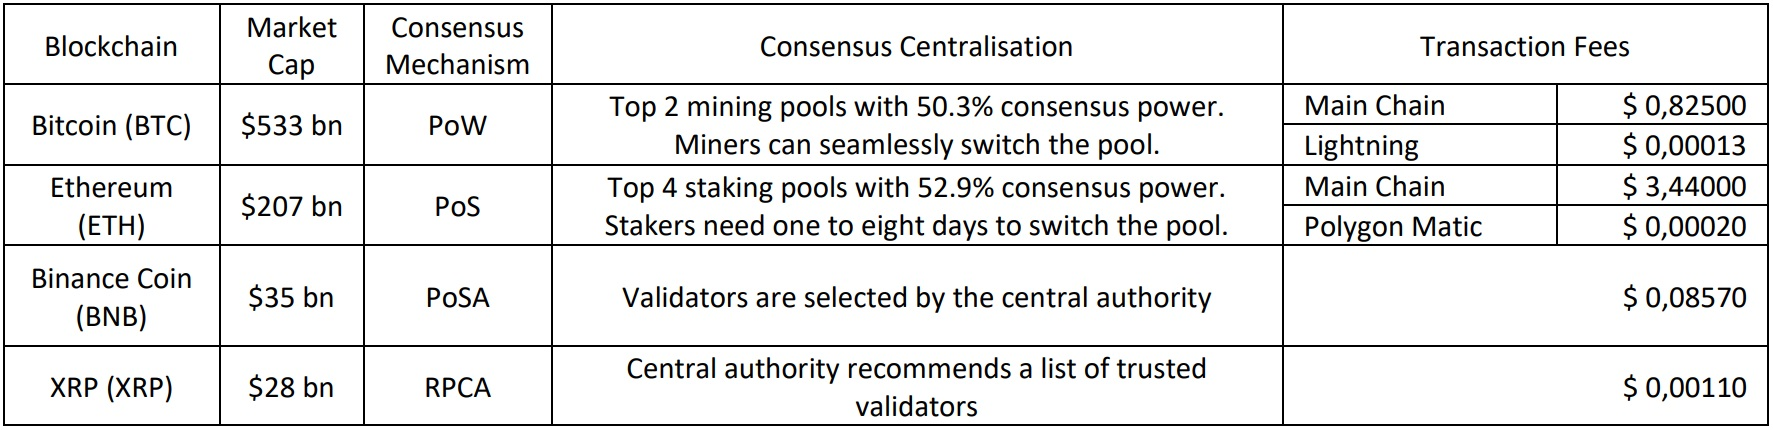
\includegraphics[width=0.9\linewidth]{Blockchains_comparison.jpg}
    \label{tab:Comparative} 
\end{figure*}


Considering the abovementioned factors (Table \ref{tab:Comparative}) and given that Bitcoin is the most accepted cryptocurrency globally (\cite{davis_cryptocurrency_2023}; \cite{flynn_how_2022}; \cite{mallqui_predicting_2019}; \cite{vejacka_basic_2014}), the study will primarily focus on the Bitcoin network as the archetypal blockchain-based payment system.

    
\clearpage

\end{document}